\documentclass[11pt,a4paper]{article}

\usepackage{a4wide}
\usepackage{polski}

\usepackage[left=2cm,right=2cm,top=2cm,bottom=3cm]{geometry}

\usepackage[utf8]{inputenc} 

\usepackage{amsmath}
\usepackage{graphicx}

\usepackage{float}
\usepackage{relsize}
\usepackage{subcaption}
\usepackage{tabularx}

\usepackage[colorlinks=true, allcolors=blue]{hyperref}

\usepackage[skip=10pt plus1pt, indent=0pt]{parskip}
\usepackage{indentfirst}

\title{Bazy danych 2 \\
Dokumentacja projektu}
\author{Dominika Boguszewska \\
Piotr Lenczewski \\
Michał Machnikowski \\
Jakub Pęk \\
Tomasz Truszkowski}
\date{Semestr 24L}

\begin{document}

\maketitle

\tableofcontents

\newpage

\section{Temat projektu}

Postanowiliśmy stworzyć aplikację służącą szukaniu osób w celu wspólnego uprawiania sportu. Użytkownicy mogą stworzyć wydarzenie, w którym deklarują miejsce, czas oraz interesujący ich sport. A także mogą zapisać się na wcześniej utworzone wydarzenia po wyszukaniu takich, które ich interesują.

\section{Grupa docelowa aplikacji}

Nasza aplikacja jest skierowana do osób, które są zainteresowanie aktywnością fizyczną i chcą znaleźć towarzyszy do wspólnego uprawiania sportu. A także dla organizatorów wydarzeń sportowych, którzy chcą łatwo znaleźć uczestników do organizowanych wydarzeń.

\section{Wymagania aplikacji}

\subsection{Wymagania funkcjonalne}

\begin{itemize}
    \item Użytkownik może stworzyć konto.
    \item Przy tworzeniu konta wymagane jest ustawienie silnego hasła.
    \item Po utworzeniu konta wysyłany jest email z potwierdzeniem do użytkownika.
    \item Użytkownik może zalogować się na swoje konto.
    \item Użytkownik może ustawić swoje zdjęcie profilowe.
    \item Użytkownik może dodać własne ogłoszenia z parametrami: rodzaj sportu, miejsce, czas, dodatkowy opis.
    \item Użytkownik może wyszukiwać oferty według podanych kryteriów (np. rodzaj sportu, miejsce, czas).
    \item Użytkownik może zapisać się na wydarzenie.
\end{itemize}
 
\subsection{Wymagania niefunkcjonalne}

\begin{itemize}
    \item Aplikacja działa na systemie operacyjnym Linux.
    \item Aplikacja działa na systemie operacyjnym Windows.
    \item Każda strona aplikacji musi się załadować w przeciągu 2 sekund.
    \item Email wysłany do użytkownika po utworzeniu konta musi do niego dojść w przeciągu 10 minut.
\end{itemize}

\section{Model pojęciowy (E-R)}

\begin{figure} [H]
    \centering
    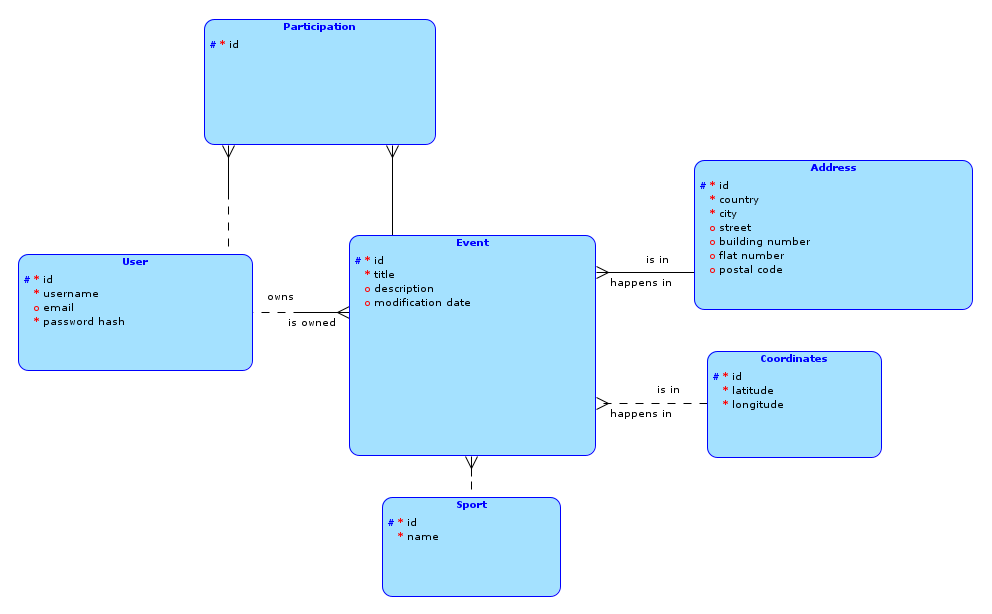
\includegraphics[width=0.95\linewidth]{model/model_er.png}
\end{figure}

\section{Model relacyjny bazy danych}

\begin{figure} [H]
    \centering
    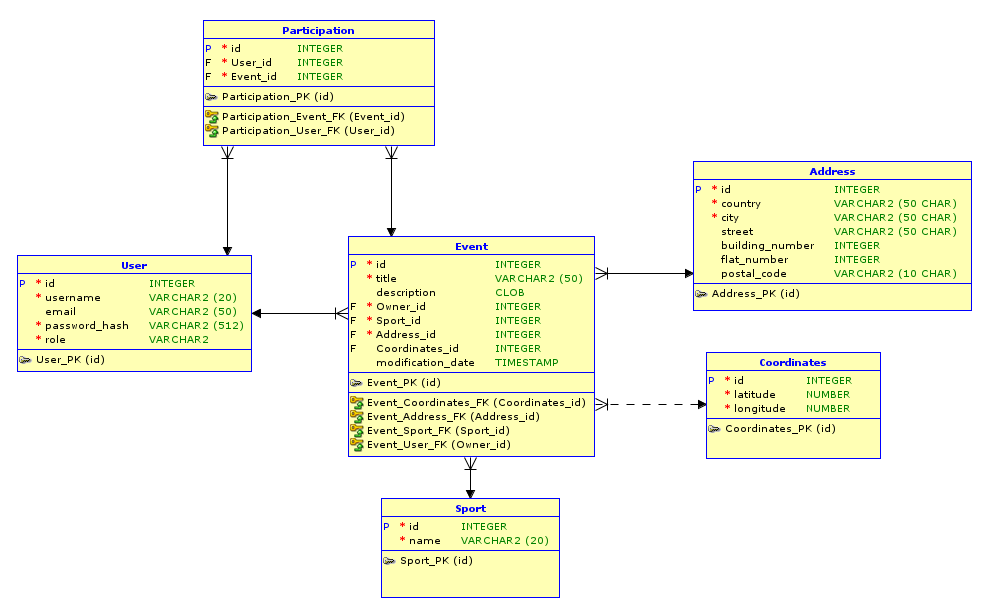
\includegraphics[width=0.95\linewidth]{model/model_rel.png}
\end{figure}

\section{Zdenormalizowany model relacyjny bazy danych}

\begin{figure} [H]
    \centering
    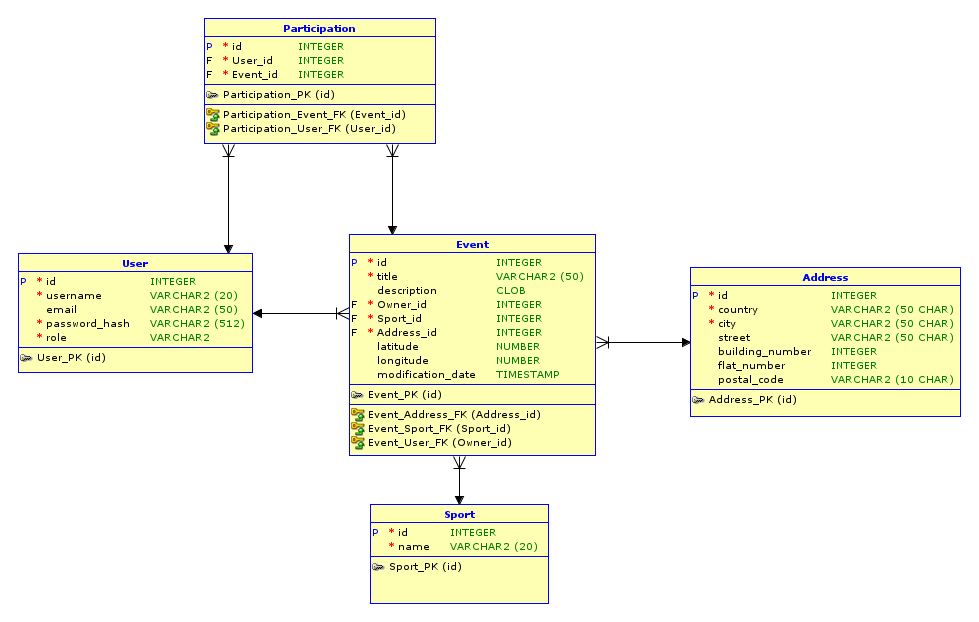
\includegraphics[width=0.95\linewidth]{model/model_denorm.png}
\end{figure}

Podczas procesu denormalizacji usunęliśmy tabelę \textit{Coordinates}, a jej atrybuty \textit{latitude} i \textit{longitude} przenieśliśmy do tabeli \textit{Event}.

\section{Wykorzystane technologie}

\begin{itemize}
    \item MySQL
    \item Java
    \item Spring Boot
    \item Next.js
\end{itemize}

\section{Instrukcja użytkowania}

\subsection{Uruchomienie aplikacji}

Po wejściu na stronę internetową uruchamia się strona powitalna, z której po kliknięciu przycisku \textit{Login} można przejść do formularzy logowania się oraz rejestracji, klikając odpowiednio przyciski \textit{Login} oraz \textit{Register}. 

\begin{figure} [H]
    \centering
    
\includegraphics[width=1\linewidth]{pages/welcome.png}
    \caption{Strona powitalna}
\end{figure}

\subsection{Logowanie się i rejestracja}

Następnie użytkownik może zalogować się na już istniejące konto bądź stworzyć nowe. W przypadku rejestracji koniecznie jest podanie silnego hasła, czyli takiego, które składa się z co najmniej 5 znaków w tym co najmniej 1 dużej litery i co najmniej 1 cyfry. Po utworzeniu nowego konta do użytkownika jest wysyłany email z potwierdzeniem pomyślnej rejestracji.

\begin{figure}[H]
    \centering
    \captionsetup{justification=centering,margin=2cm}
        \begin{subfigure}{0.49\textwidth}
            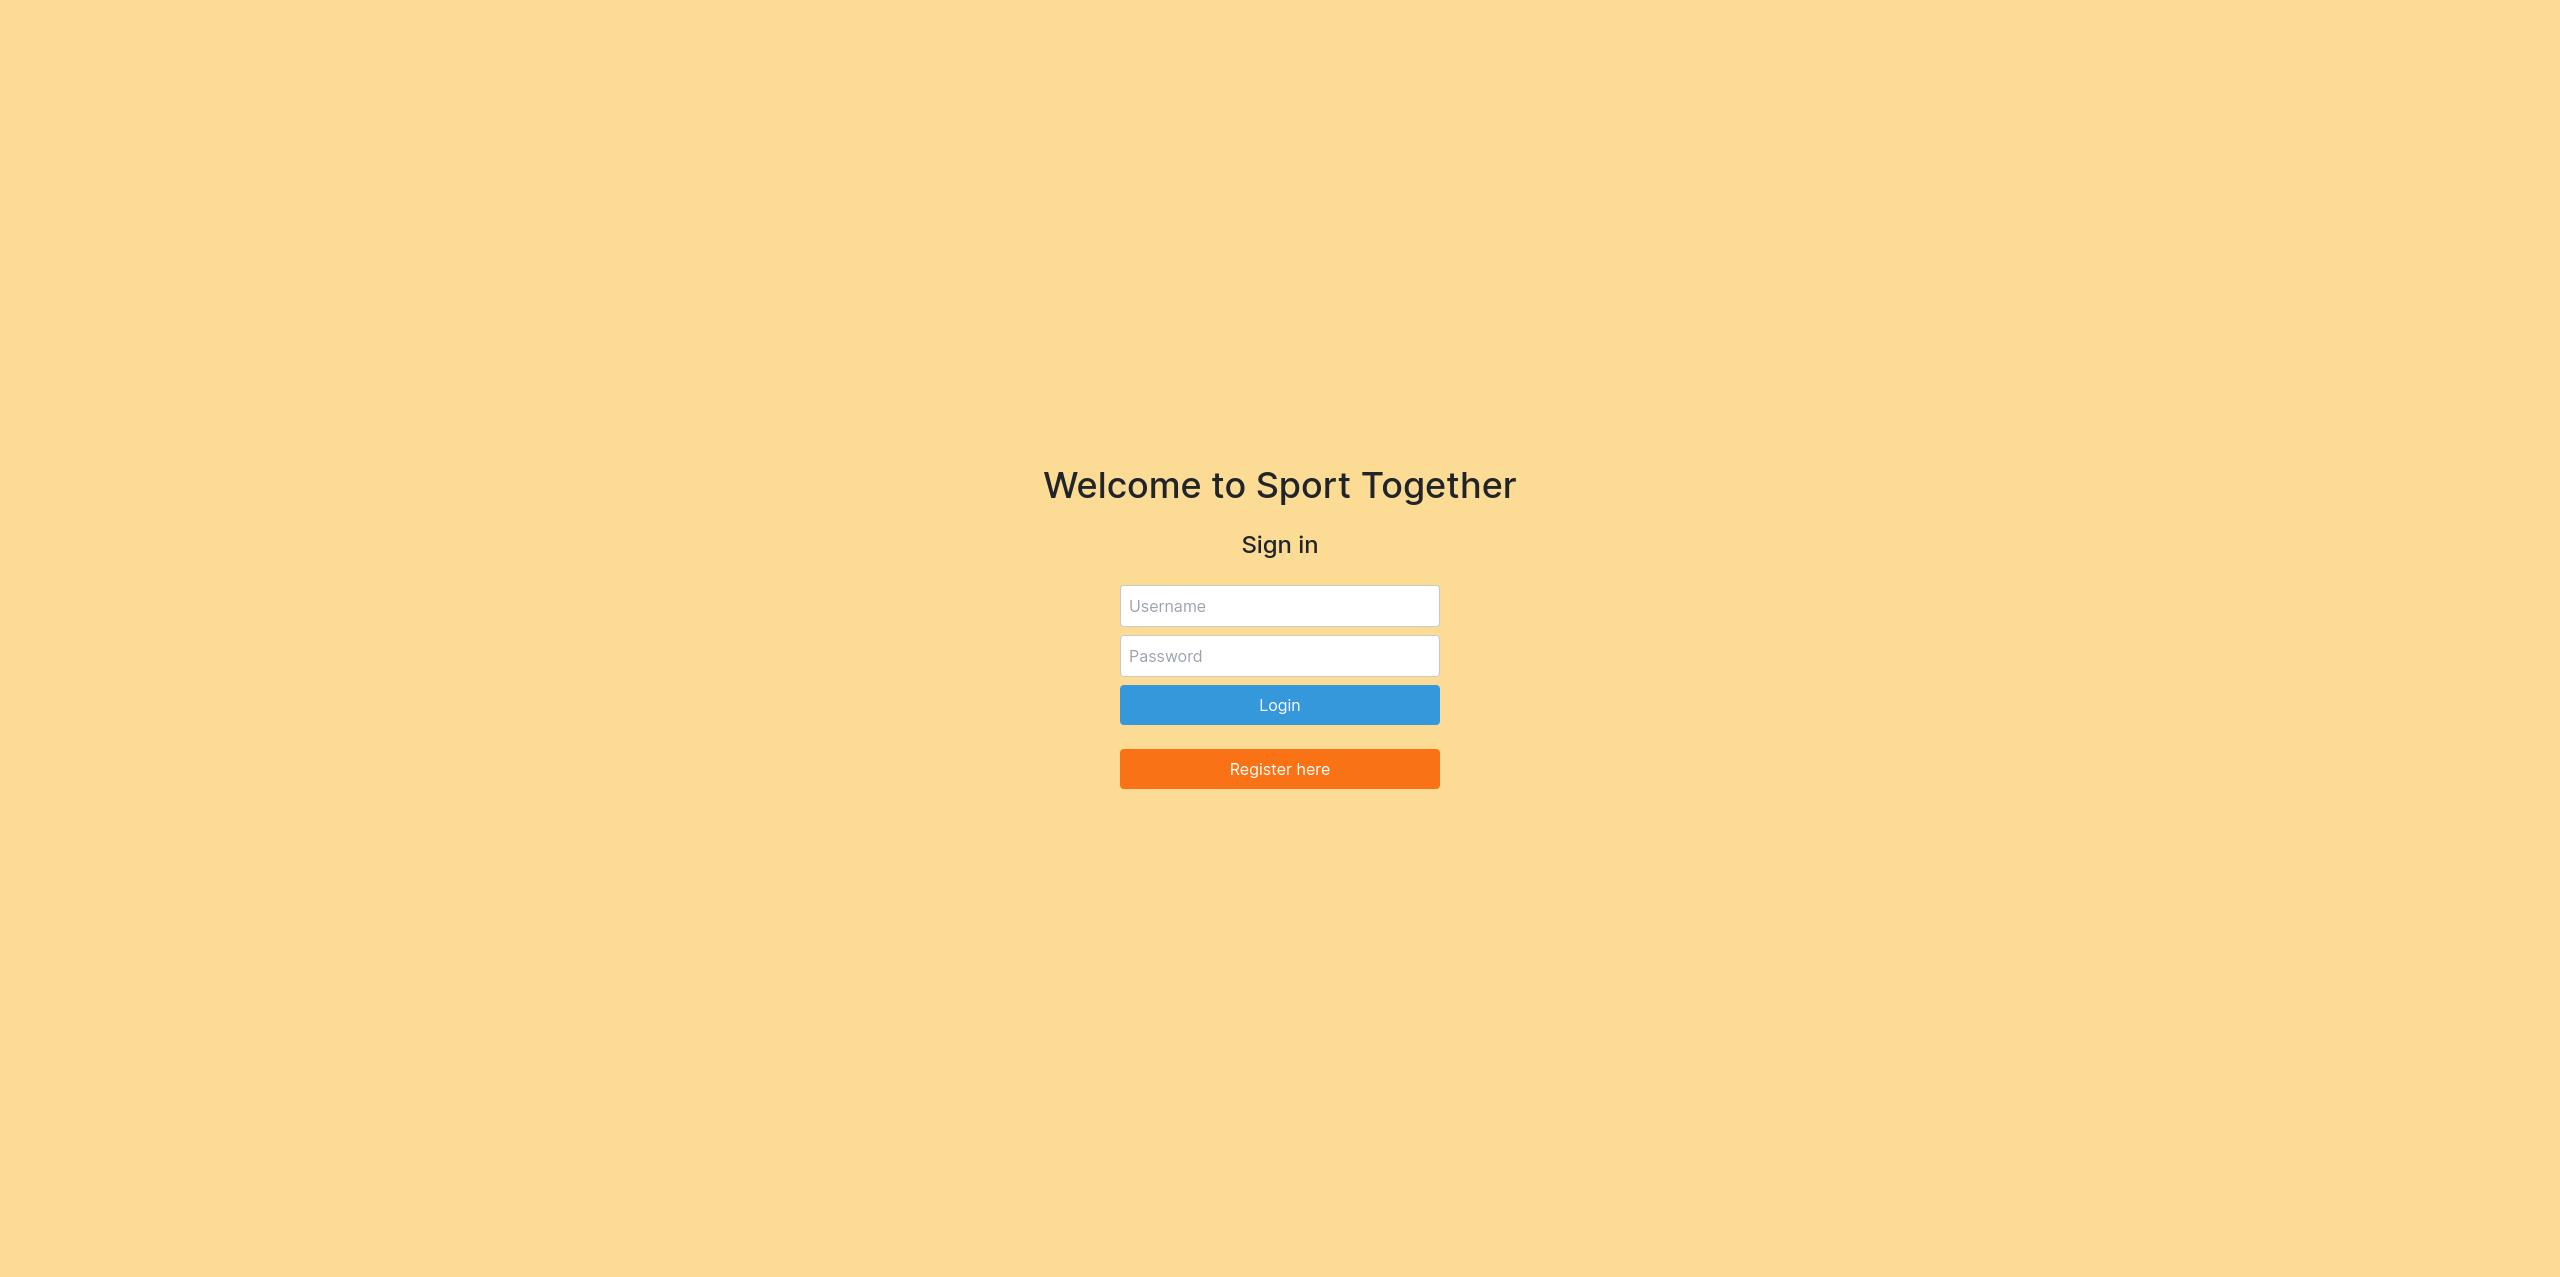
\includegraphics[width=\textwidth]{pages/login_page.png}
            \caption{Formularz logowania się}
        \end{subfigure}
    \hfill
        \begin{subfigure}{0.49\textwidth}
            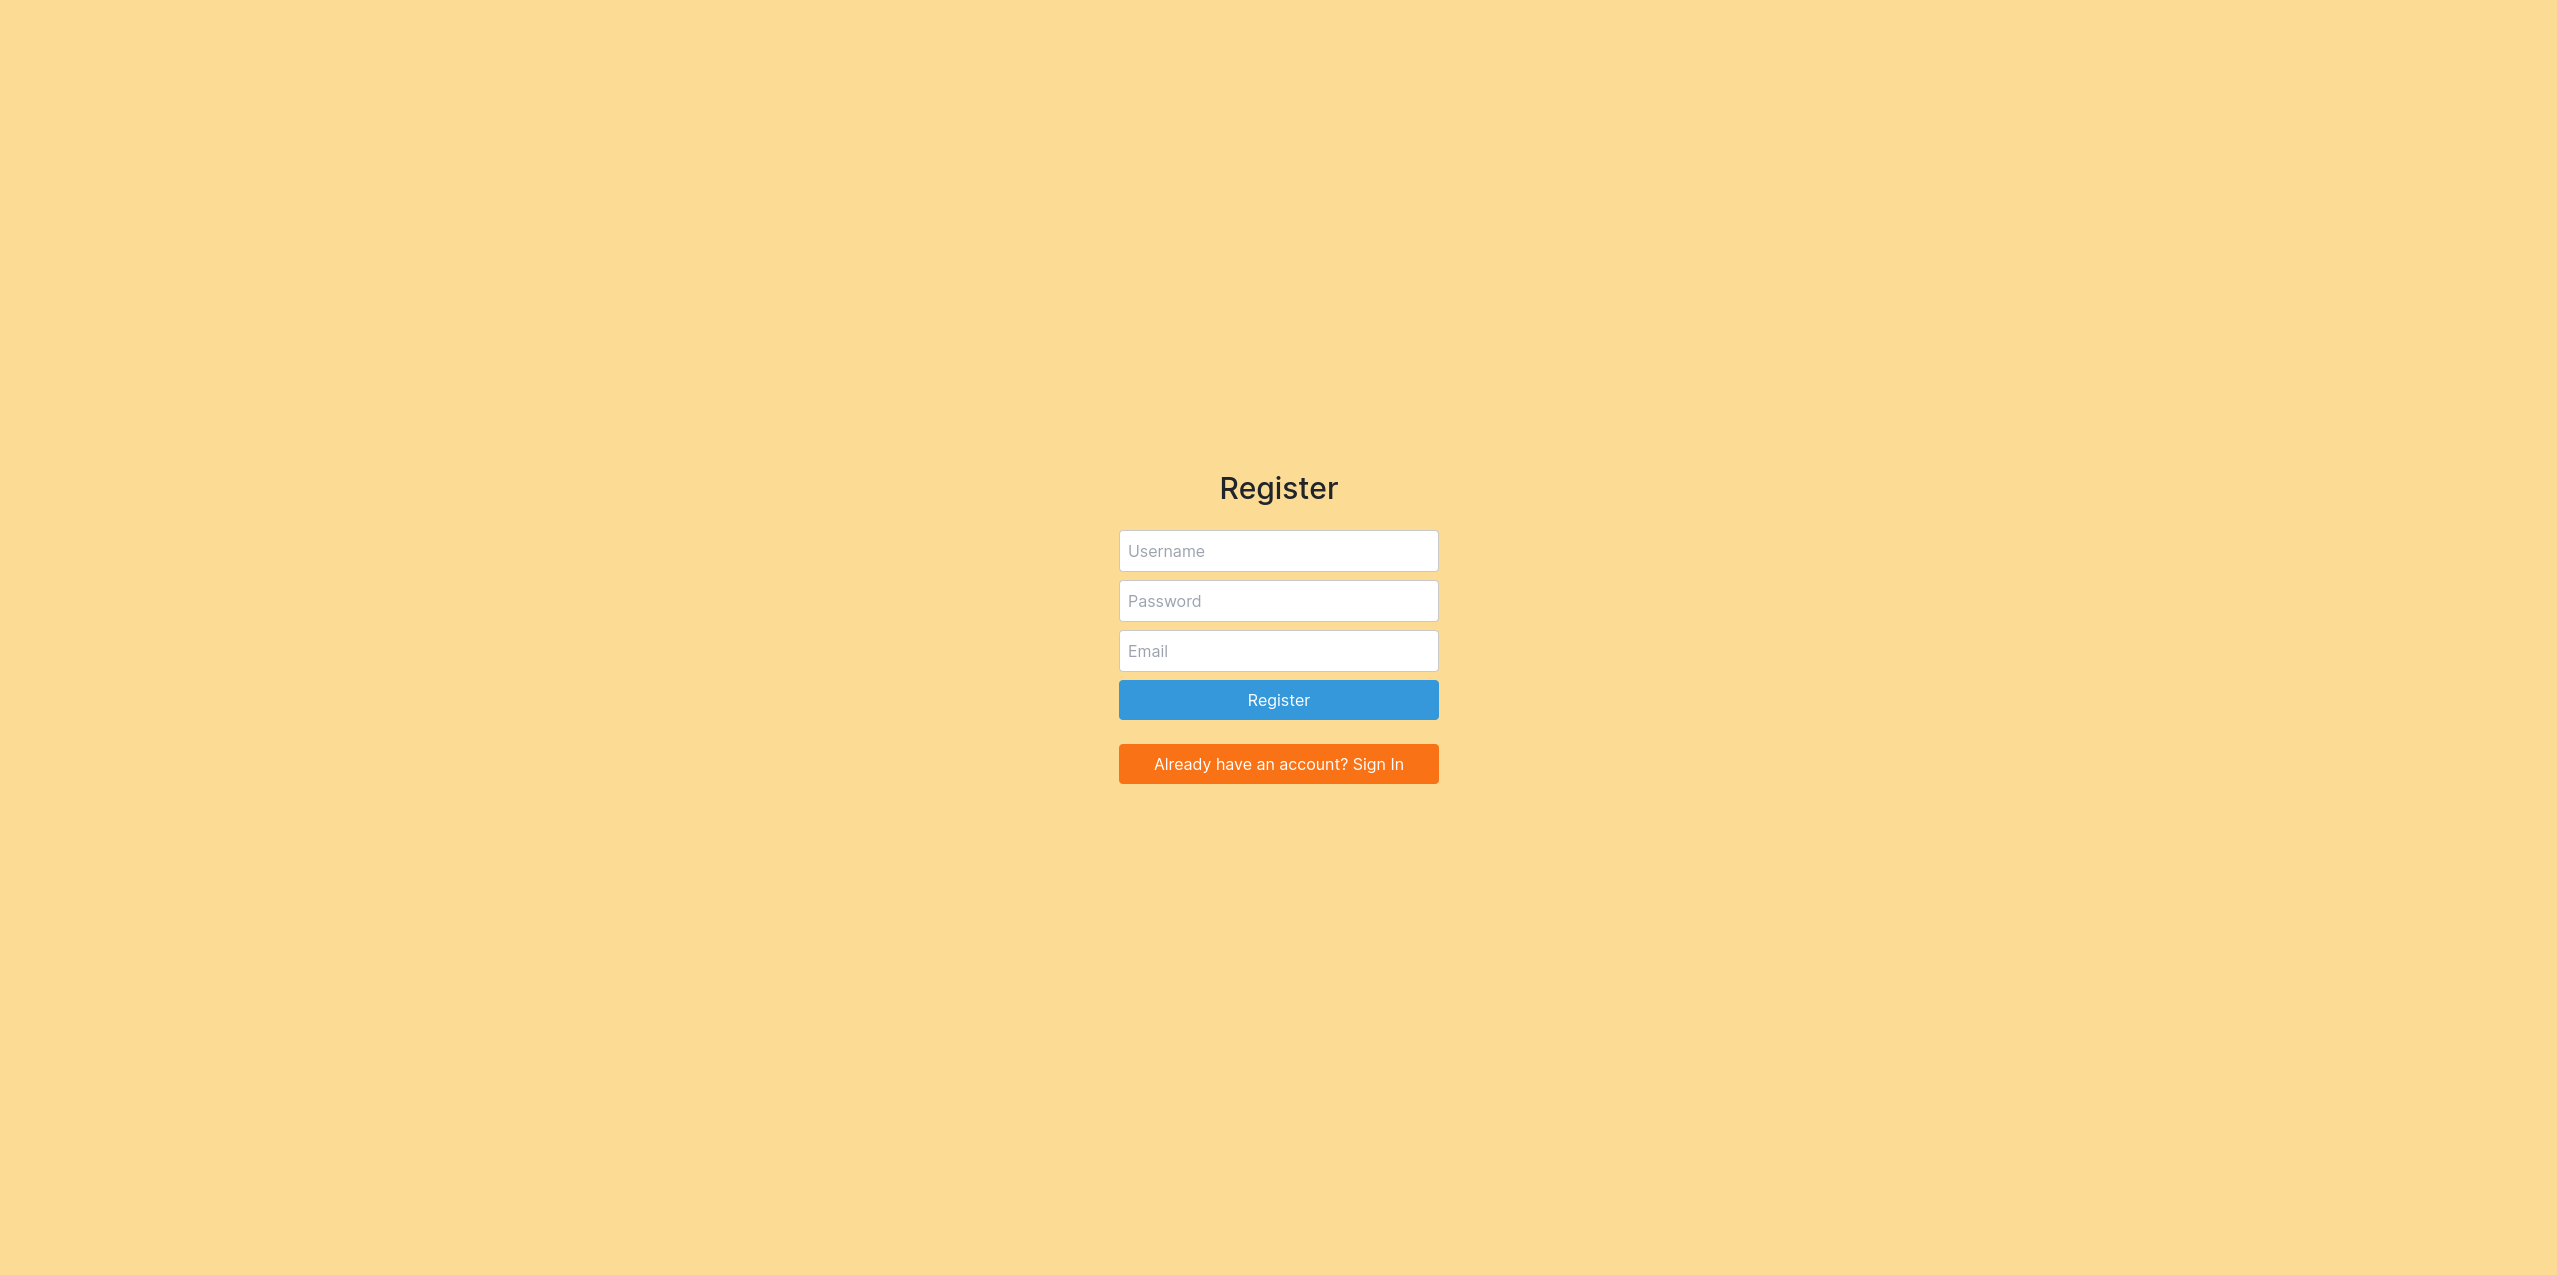
\includegraphics[width=\textwidth]{pages/register.png}
            \caption{Formularz rejestracji}
        \end{subfigure}
\end{figure}

\begin{figure} [H]
    \centering
    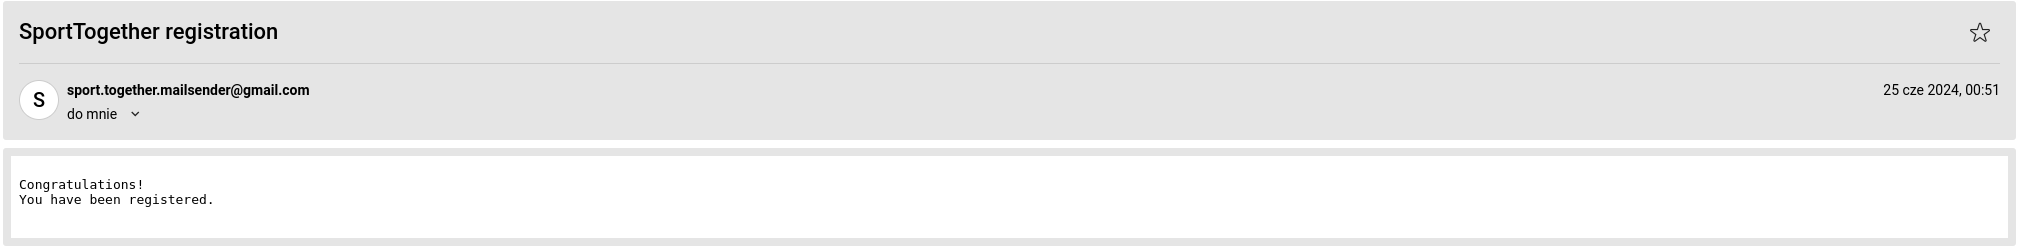
\includegraphics[width=1\linewidth]{pages/email.png}
    \caption{Email potwierdzający pomyślną rejestrację}
\end{figure}

\subsection{Strona główna}

Po tym zostaje przeniesiony na stronę główną, gdzie są wyświetlane wydarzenia, w których uczestniczy oraz te, które organizuje. Może także stamtąd przejść na stronę służącą wyszukiwaniu wydarzeń, wyświetlić informacje o swoim koncie, przejść do formularza tworzenia nowego wydarzenia lub się wylogować.

\begin{figure} [H]
    \centering
    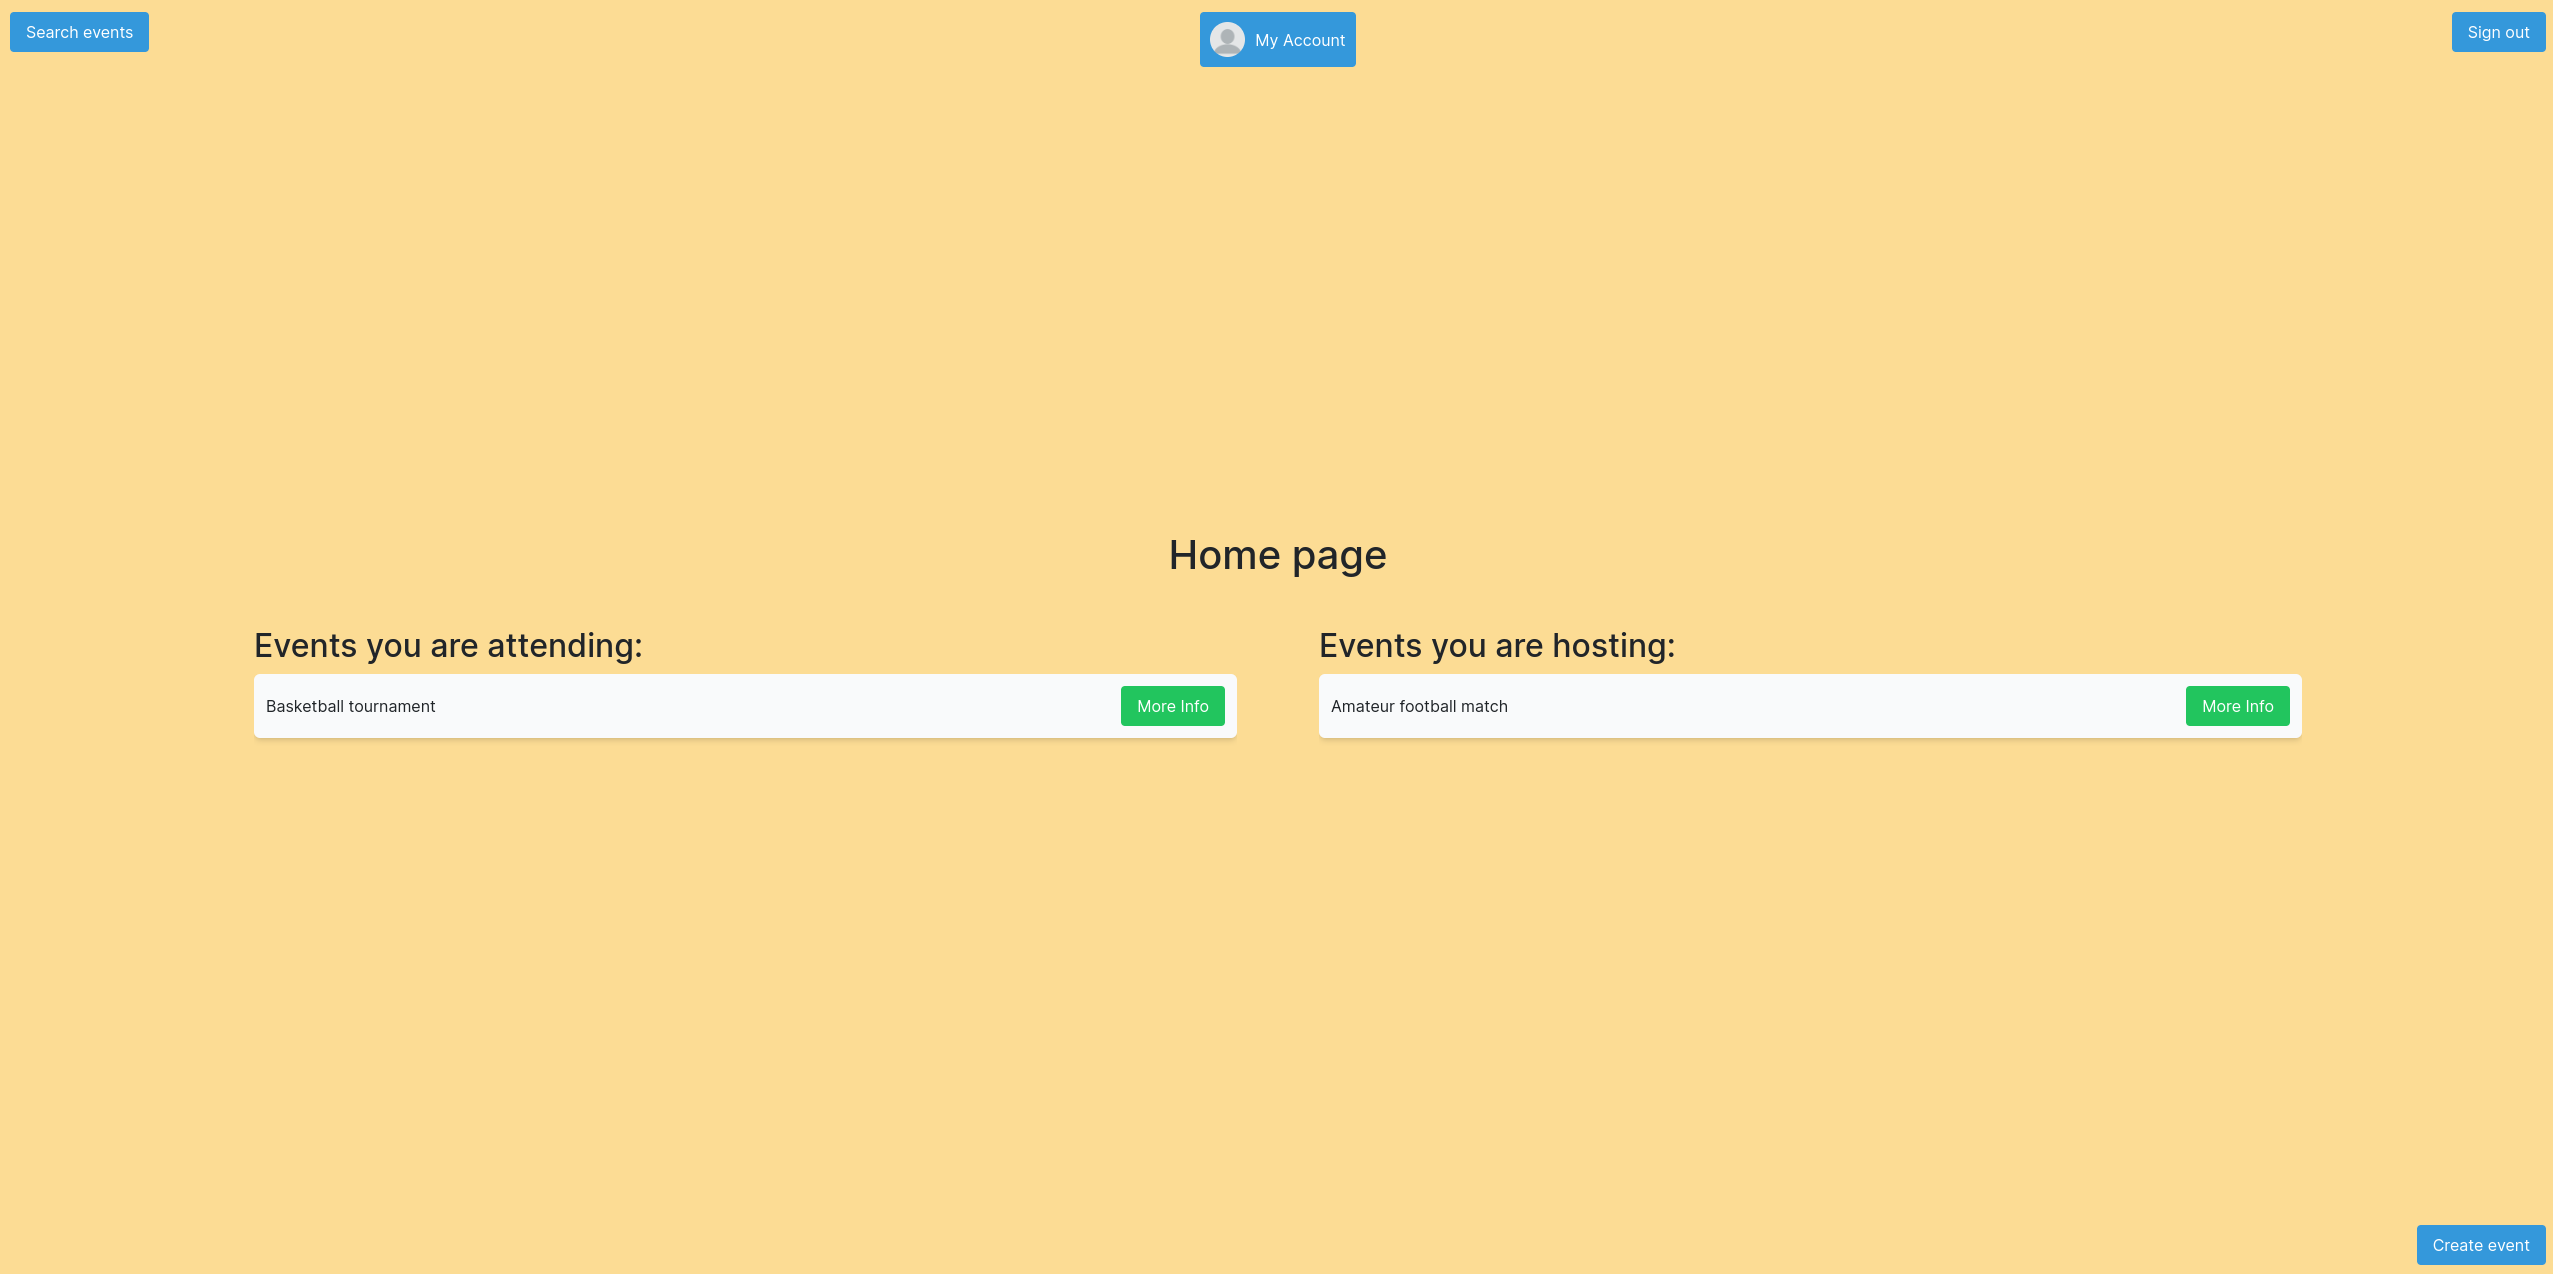
\includegraphics[width=1\linewidth]{pages/home.png}
    \caption{Strona główna}
\end{figure}

\subsection{Profil użytkownika}

Po kliknięciu przycisku \textit{My Account} na stronie głównej, użytkownik zostaje przeniesiony na stronę swojego profilu, gdzie za pomocą przycisku \textit{Upload Profile Picture} może zmienić swoje zdjęcie profilowe.

\begin{figure}[H]
    \centering
    \captionsetup{justification=centering,margin=2cm}
        \begin{subfigure}{0.49\textwidth}
            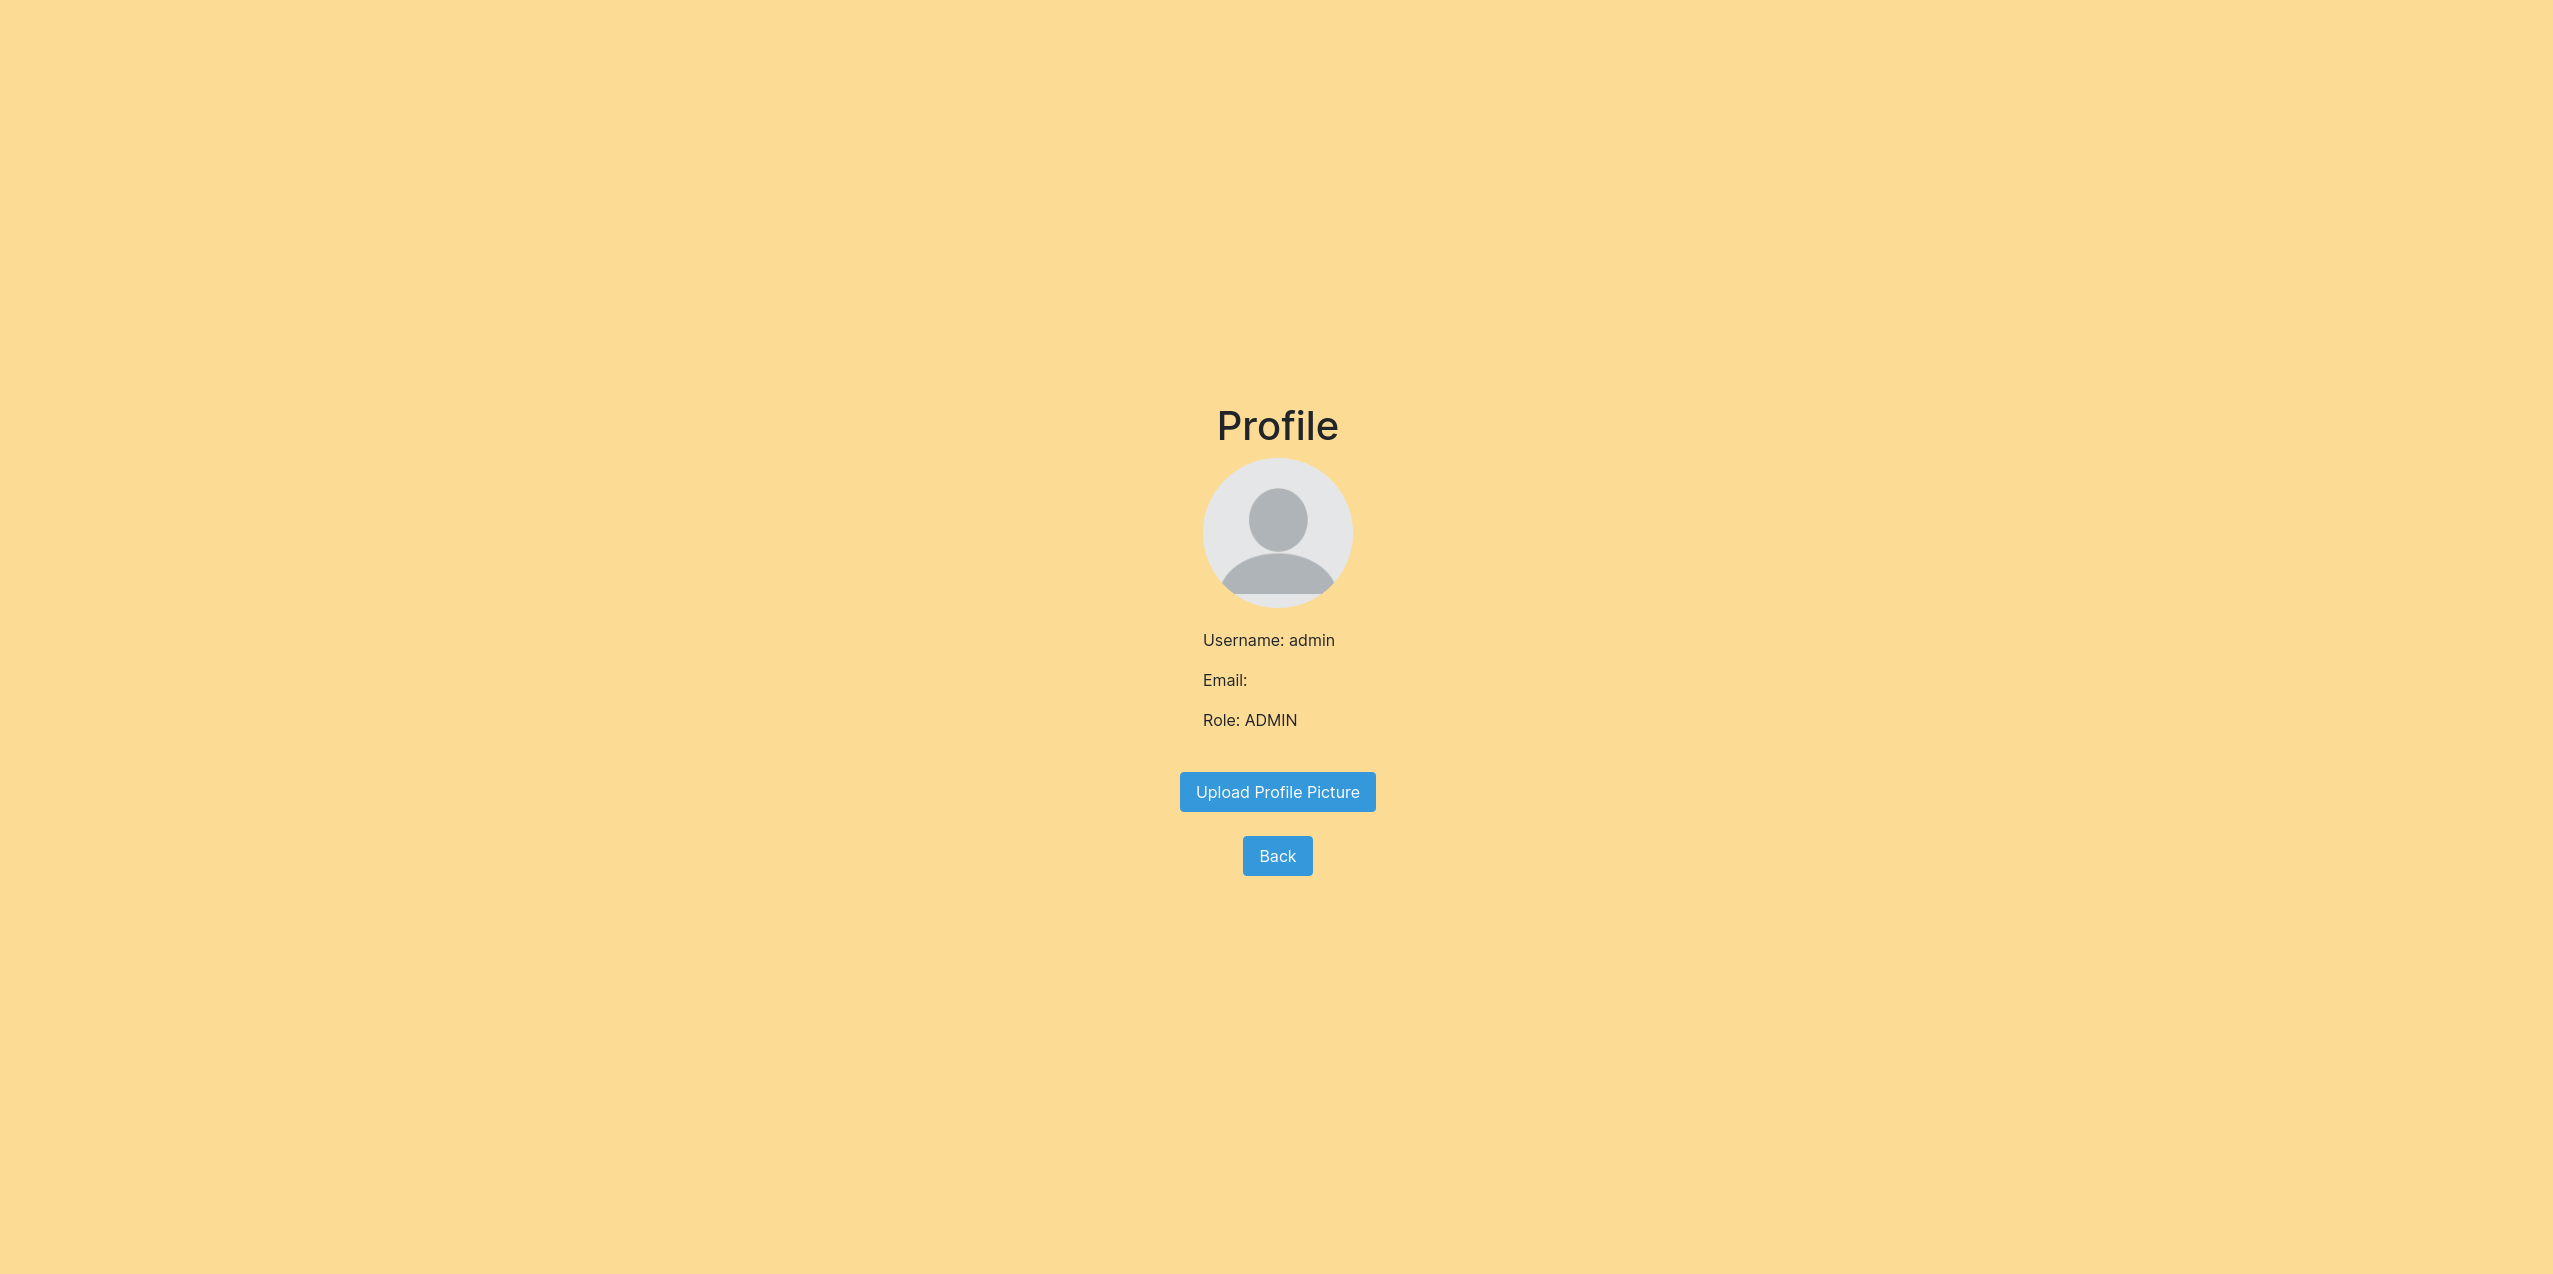
\includegraphics[width=\textwidth]{pages/account.png}
            \caption{Profil użytkownika z domyślnym zdjęciem profilowym}
        \end{subfigure}
    \hfill
        \begin{subfigure}{0.49\textwidth}
            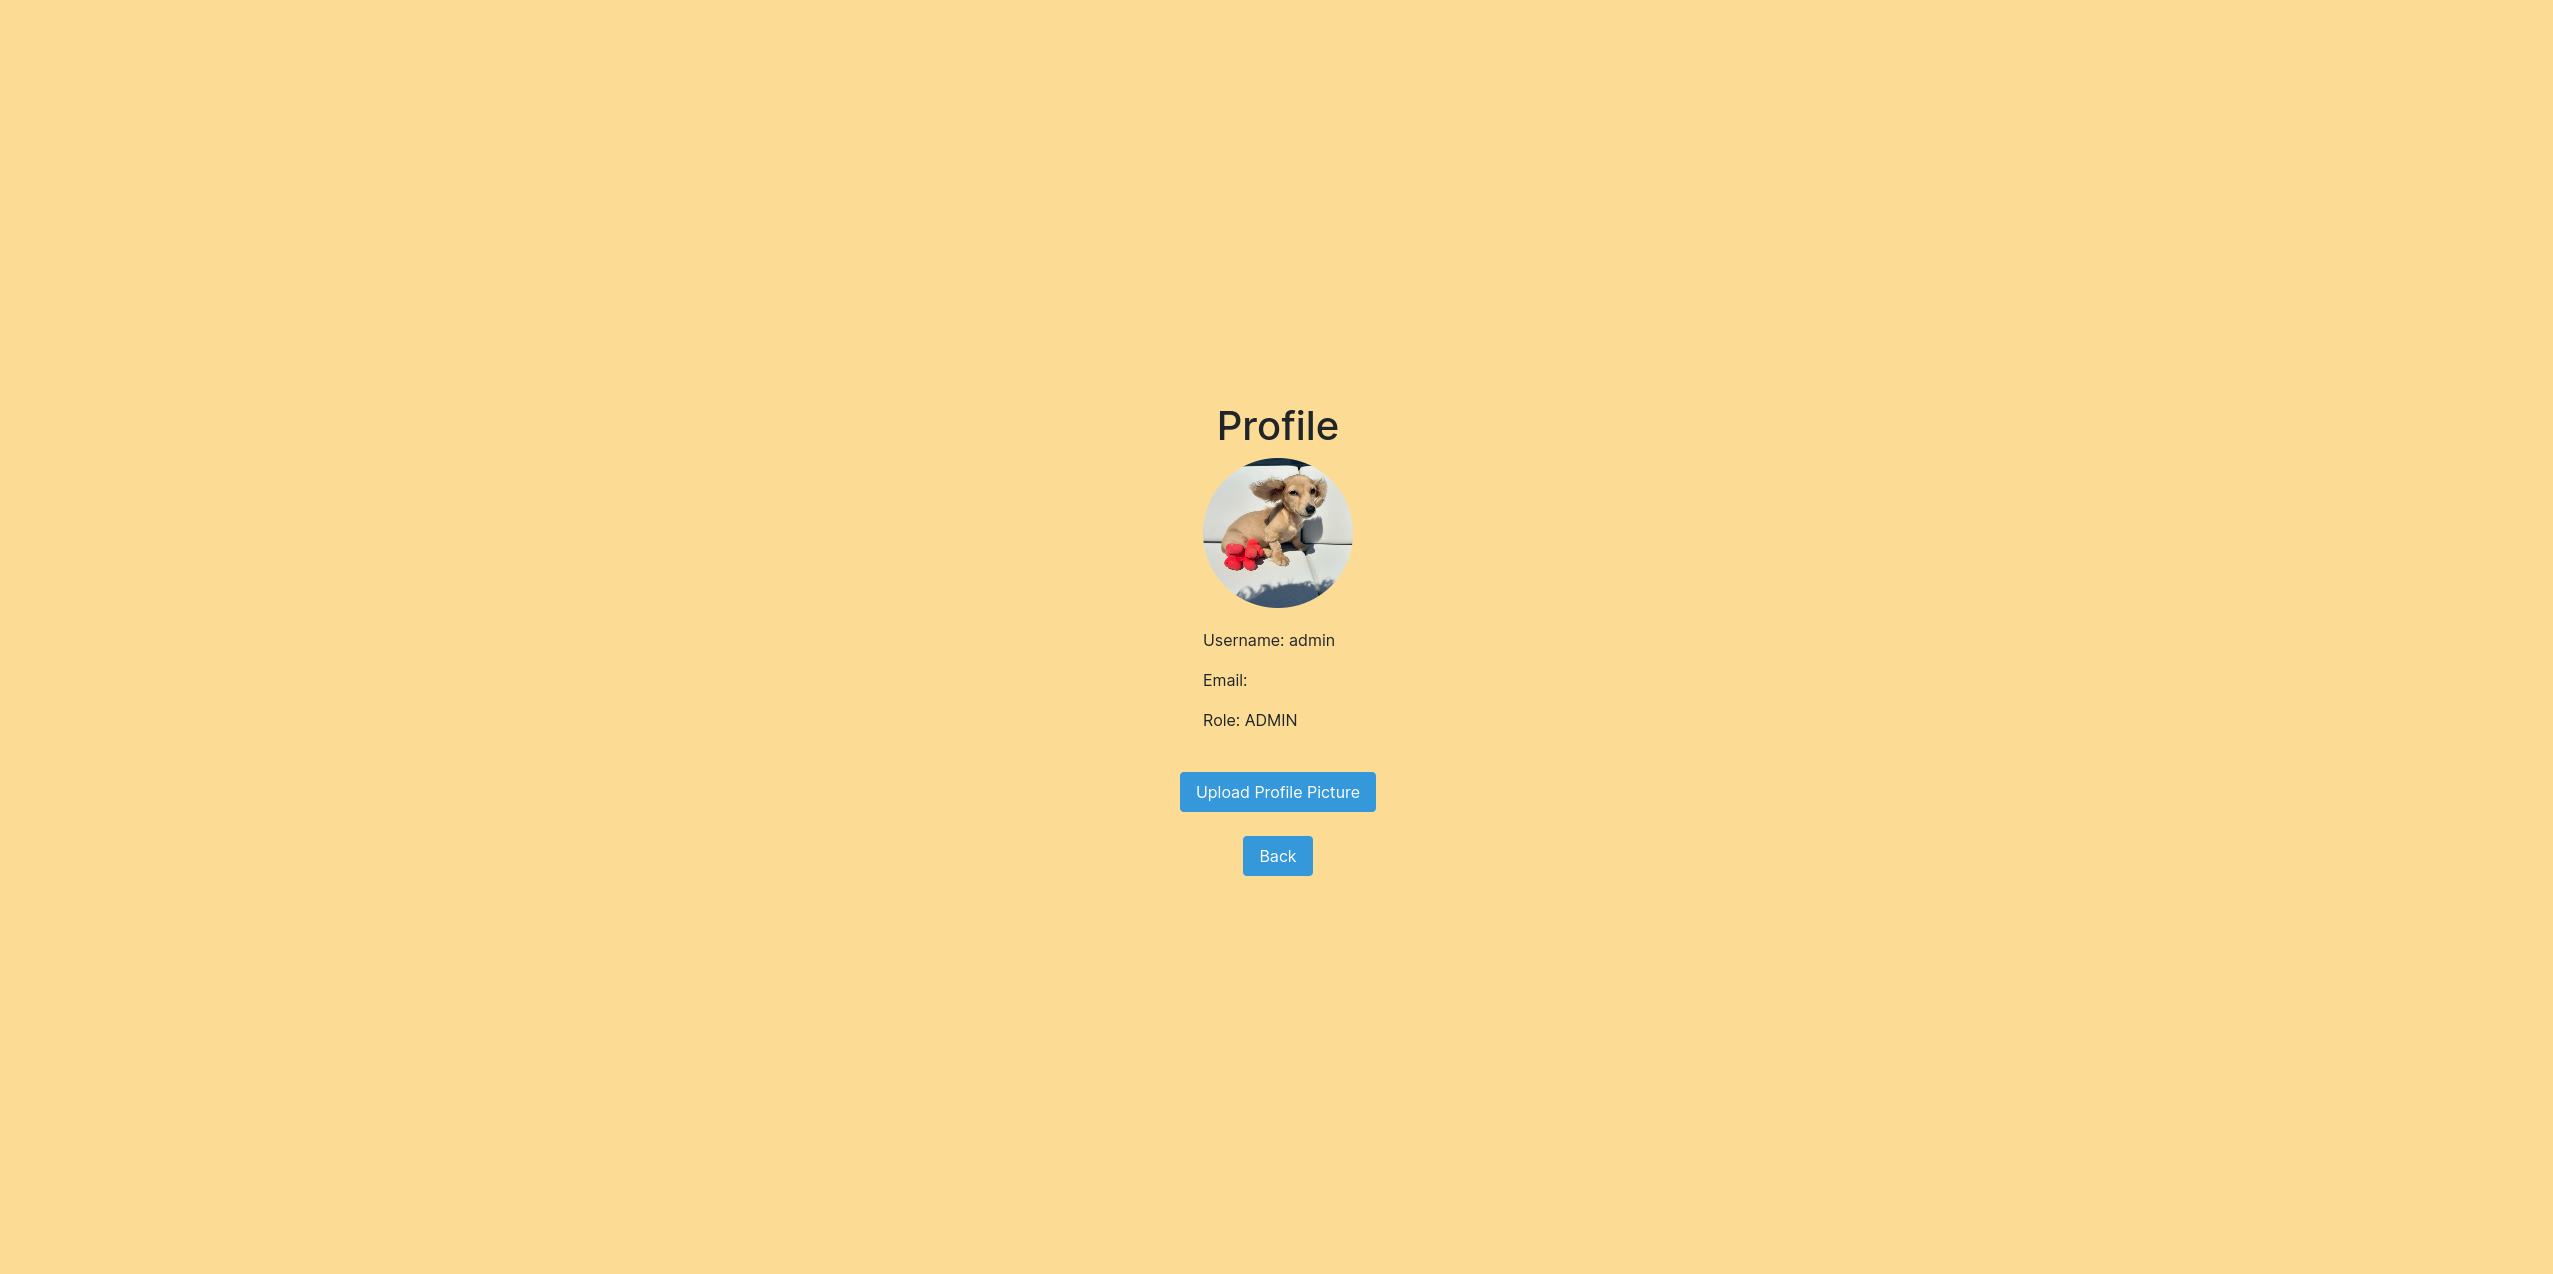
\includegraphics[width=\textwidth]{pages/account_with_profile_picture.png}
            \caption{Profil użytkownika z własnym zdjęciem profilowym}
        \end{subfigure}
\end{figure}

\subsection{Wyszukiwanie wydarzeń}

Po kliknięciu przycisku \textit{Search events} na stronie głównej, użytkownik zostaje przeniesiony na stronę służącą wyszukiwaniu wydarzeń sportowych. Domyślnie są wyświetlane wszystkie dostępne wydarzenia, na które użytkownik nie jest zapisany lub których nie organizuje, ale dzięki paskowi wyszukiwania można filtrować wydarzenia po interesującym użytkownika mieście, a dzięki checkboxom można filtrować wydarzenia po interesujących użytkownika sportach.

\begin{figure} [H]
    \centering
    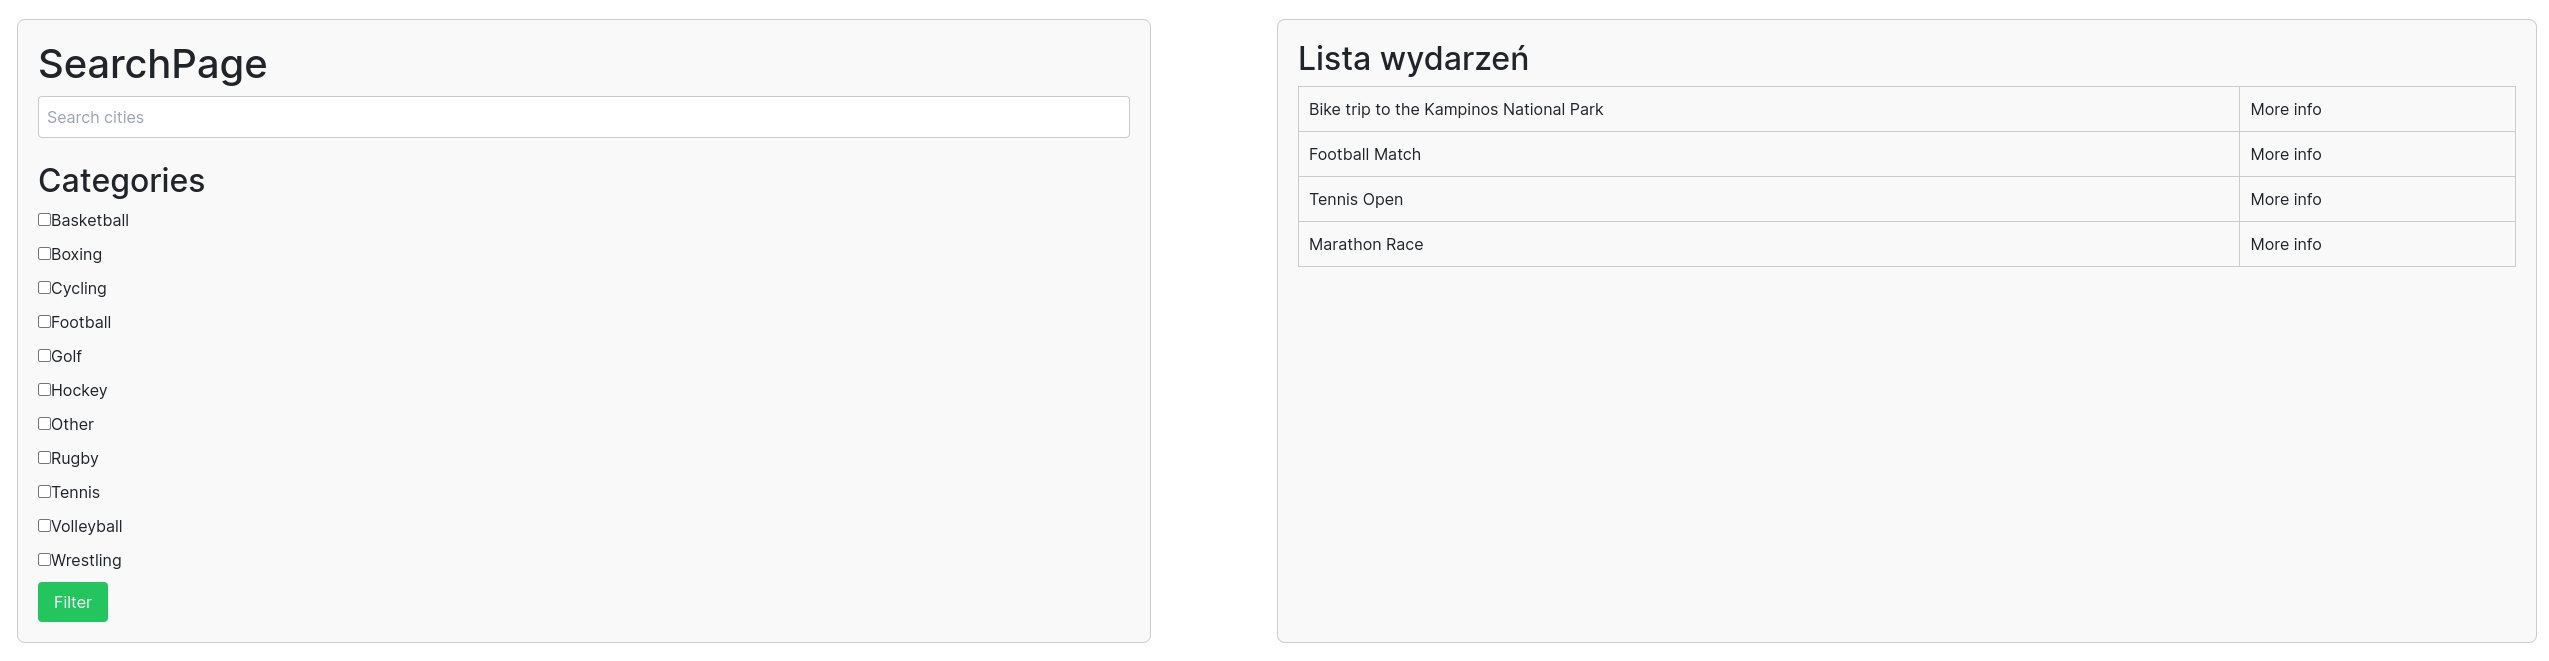
\includegraphics[width=1\linewidth]{pages/search_events.png}
    \caption{Wyszukiwanie wydarzeń}
\end{figure}

\subsection{Zapisywanie się na wydarzenia}

Po kliknięciu przycisku \textit{More info} obok tytułu wydarzenia, użytkownik zostaje przeniesiony na stronę wybranego wydarzenia. Może stamtąd odczytać szczegółowe informacje o wydarzeniu takie jak: opis wydarzenia, rodzaj sportu, login organizatora, miejsce wydarzenia, czas rozpoczęcia i zakończenia oraz datę ostatniej modyfikacji. Z tej strony użytkownik także może zapisać się na owe wydarzenie poprzez kliknięcie przycisku \textit{Join Event}, po czym zostanie ukazany popup informujący o pomyślnym zapisu się oraz użytkownik zostanie przeniesiony na stronę główną.

\begin{figure} [H]
    \centering
    
\includegraphics[width=1\linewidth]{pages/event.png}
    \caption{Strona wydarzenia}
\end{figure}

\subsection{Wypisywanie się z wydarzenia}

Aby wypisać się z wydarzenia, należy wejść w jego szczegóły ze strony głównej (z sekcji \textit{Events you are attending}), a następnie kliknąć przycisk \textit{Leave Event}. Analogicznie jak w przypadku zapisywania się, zostanie ukazany popup informujący o pomyślnym wypisaniu się i użytkownik zostanie przeniesiony na stronę główną.

\begin{figure} [H]
    \centering
    
\includegraphics[width=1\linewidth]{pages/event_leave.png}
    \caption{Strona wydarzenia}
\end{figure}

\subsection{Tworzenie nowych wydarzeń}

Po kliknięciu przycisku \textit{Create event} na stronie głównej, użytkownik zostaje przeniesiony na stronę służącą tworzeniu wydarzeń. Po wypełnieniu pól formularza i kliknięciu przycisku \textit{Add Event}, wydarzenie zostanie utworzone, a użytkownik zostanie przeniesiony na stronę główną.

\begin{figure} [H]
    \centering
    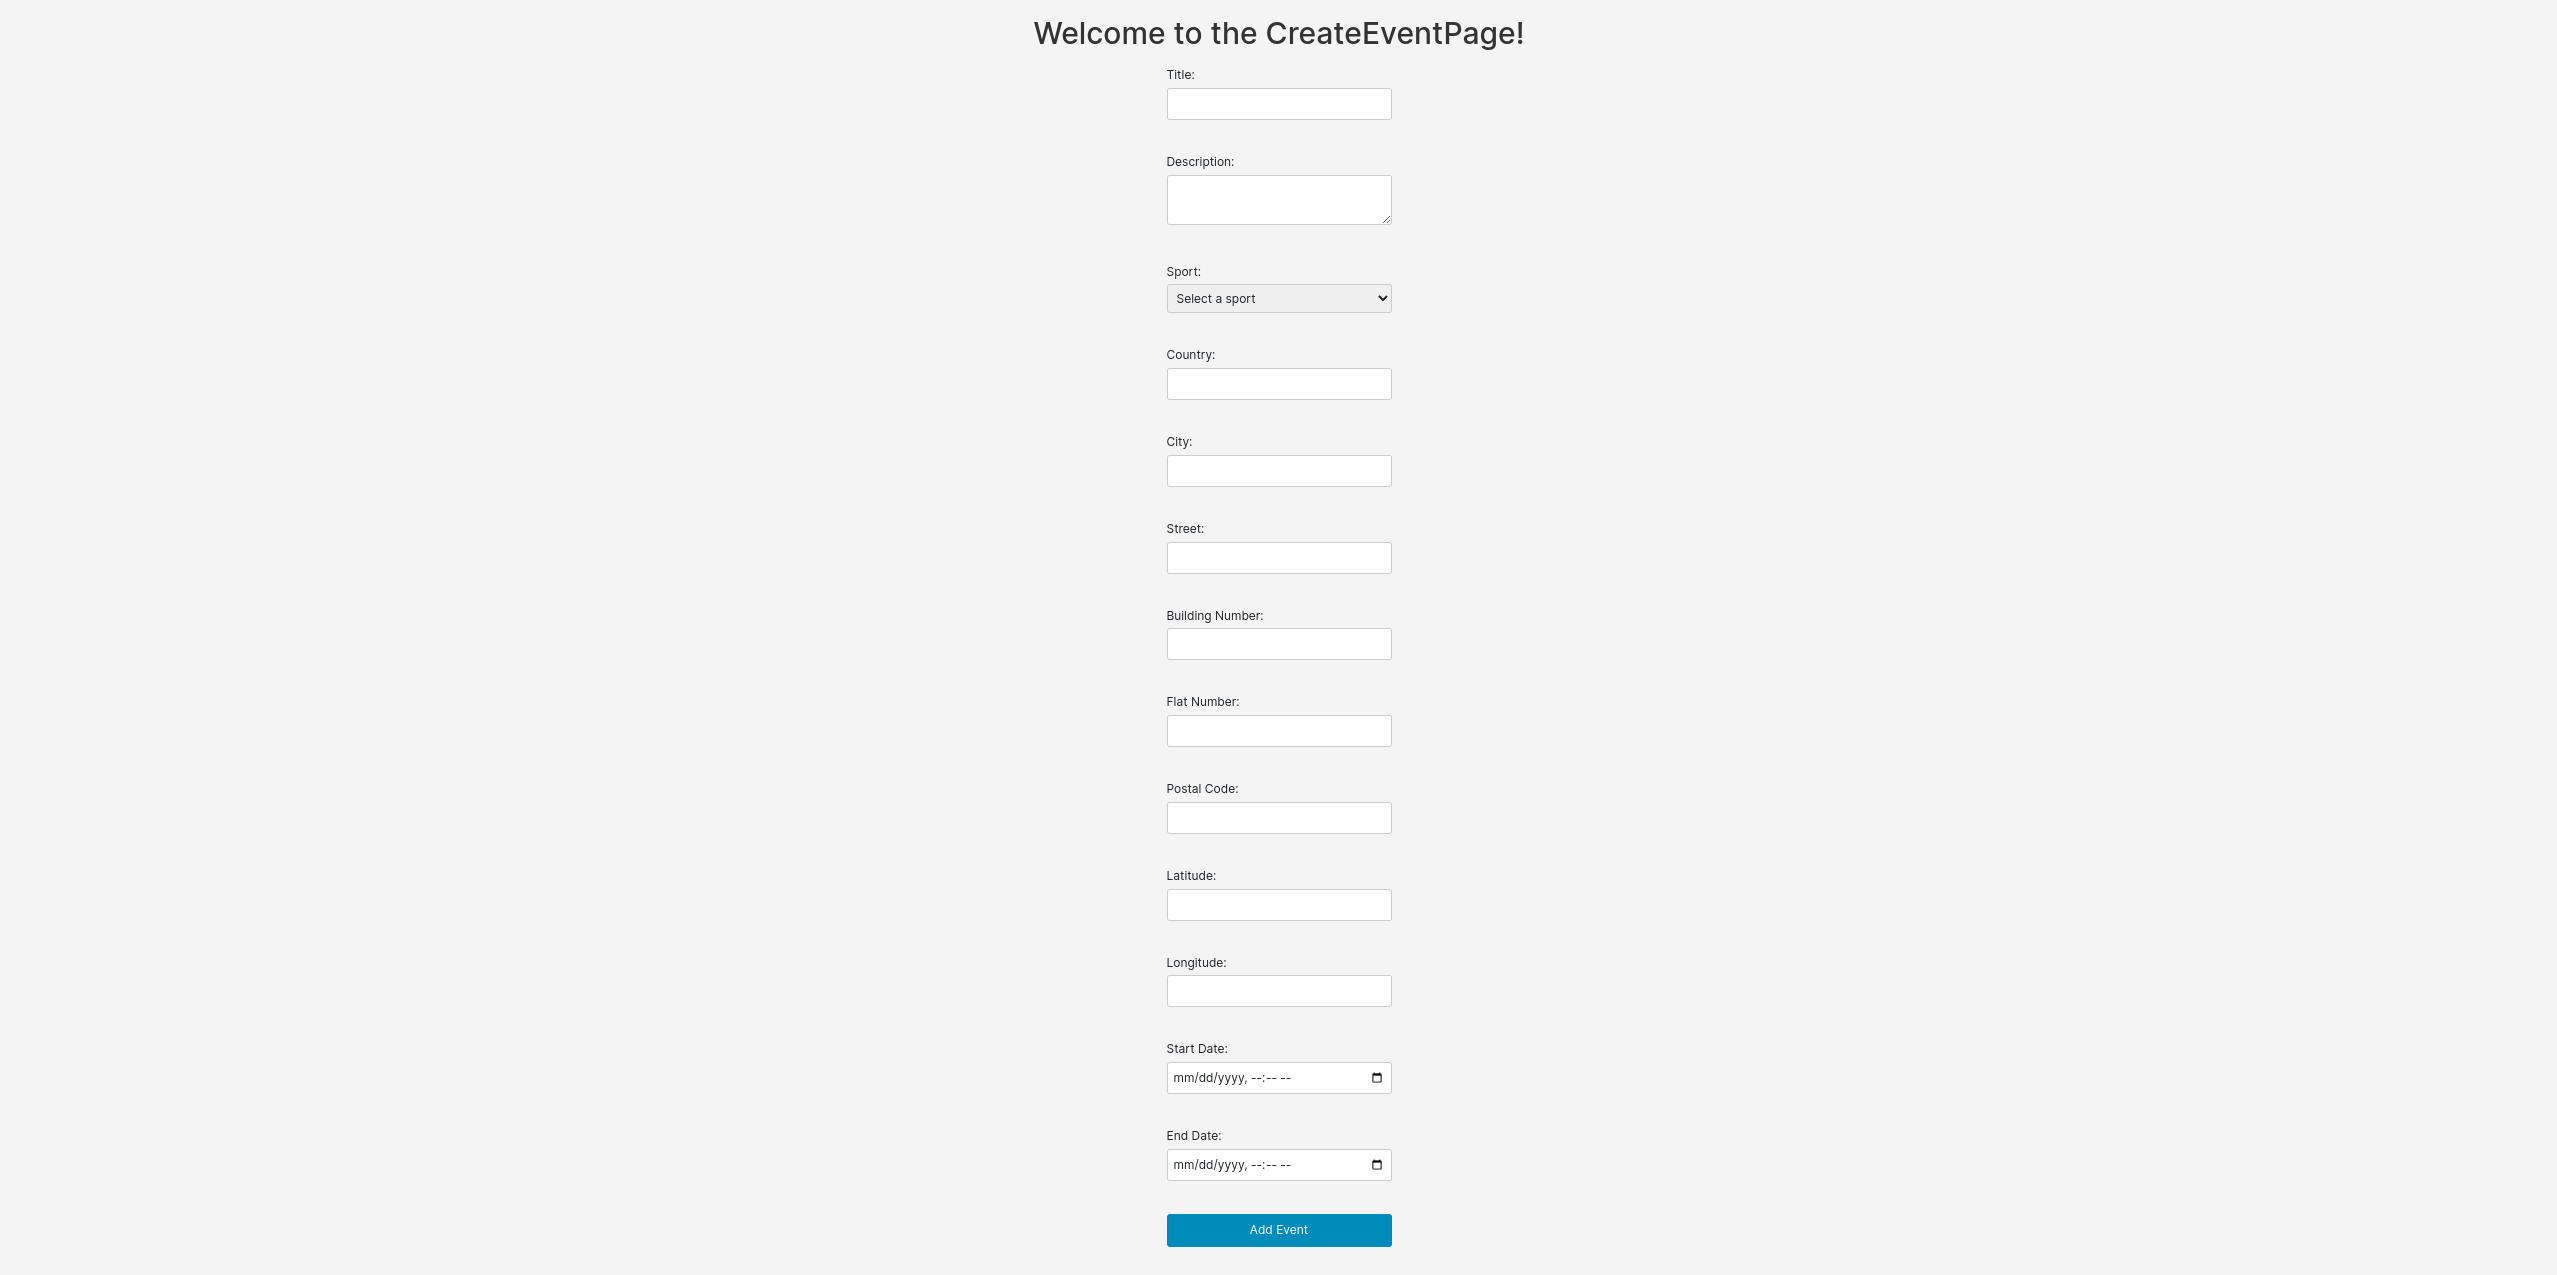
\includegraphics[width=1\linewidth]{pages/create_event.png}
    \caption{Formularz służący tworzeniu wydarzeń sportowych}
\end{figure}

\subsection{Edytowanie utworzonego wydarzenia}

Aby edytować utworzone wydarzenie, należy wejść na jego stronę ze strony głównej (z sekcji \textit{Events you are hosting}), a następnie kliknąć przycisk \textit{Edit Event}. Użytkownik zostanie przeniesiony do formularza edycji wydarzenia, gdzie może zmienić jego szczegóły poprzez edycję wartości pól. Może zapisać dokonane zmiany za pomocą przycisku \textit{Save} lub je odrzucić za pomocą przycisku \textit{Discard Changes}.

\begin{figure} [H]
    \centering
    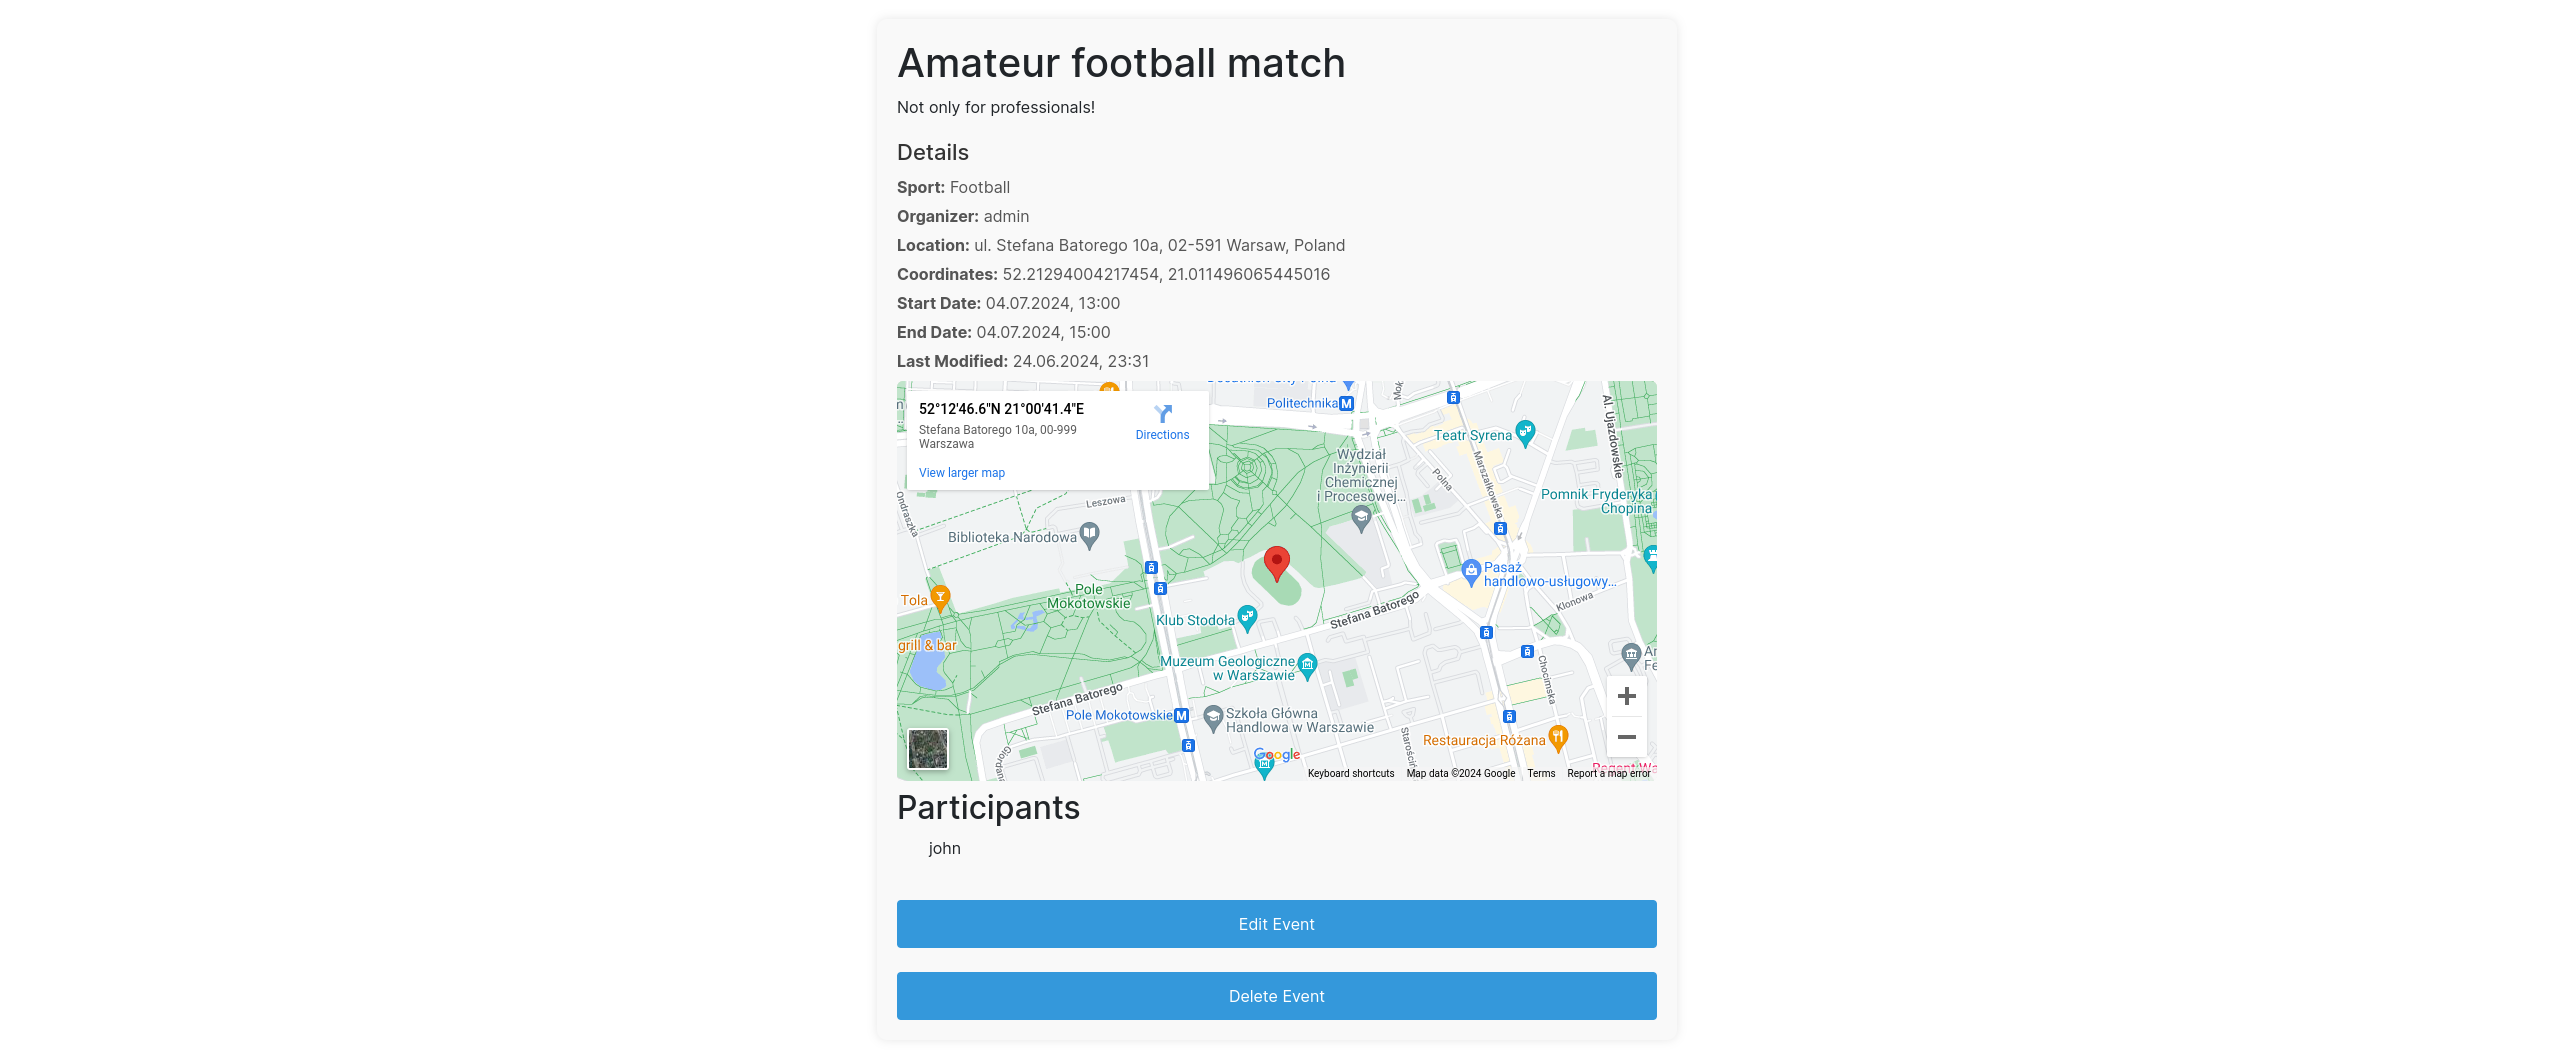
\includegraphics[width=1\linewidth]{pages/my_event.png}
    \caption{Strona utworzonego wydarzenia}
\end{figure}

\begin{figure} [H]
    \centering
    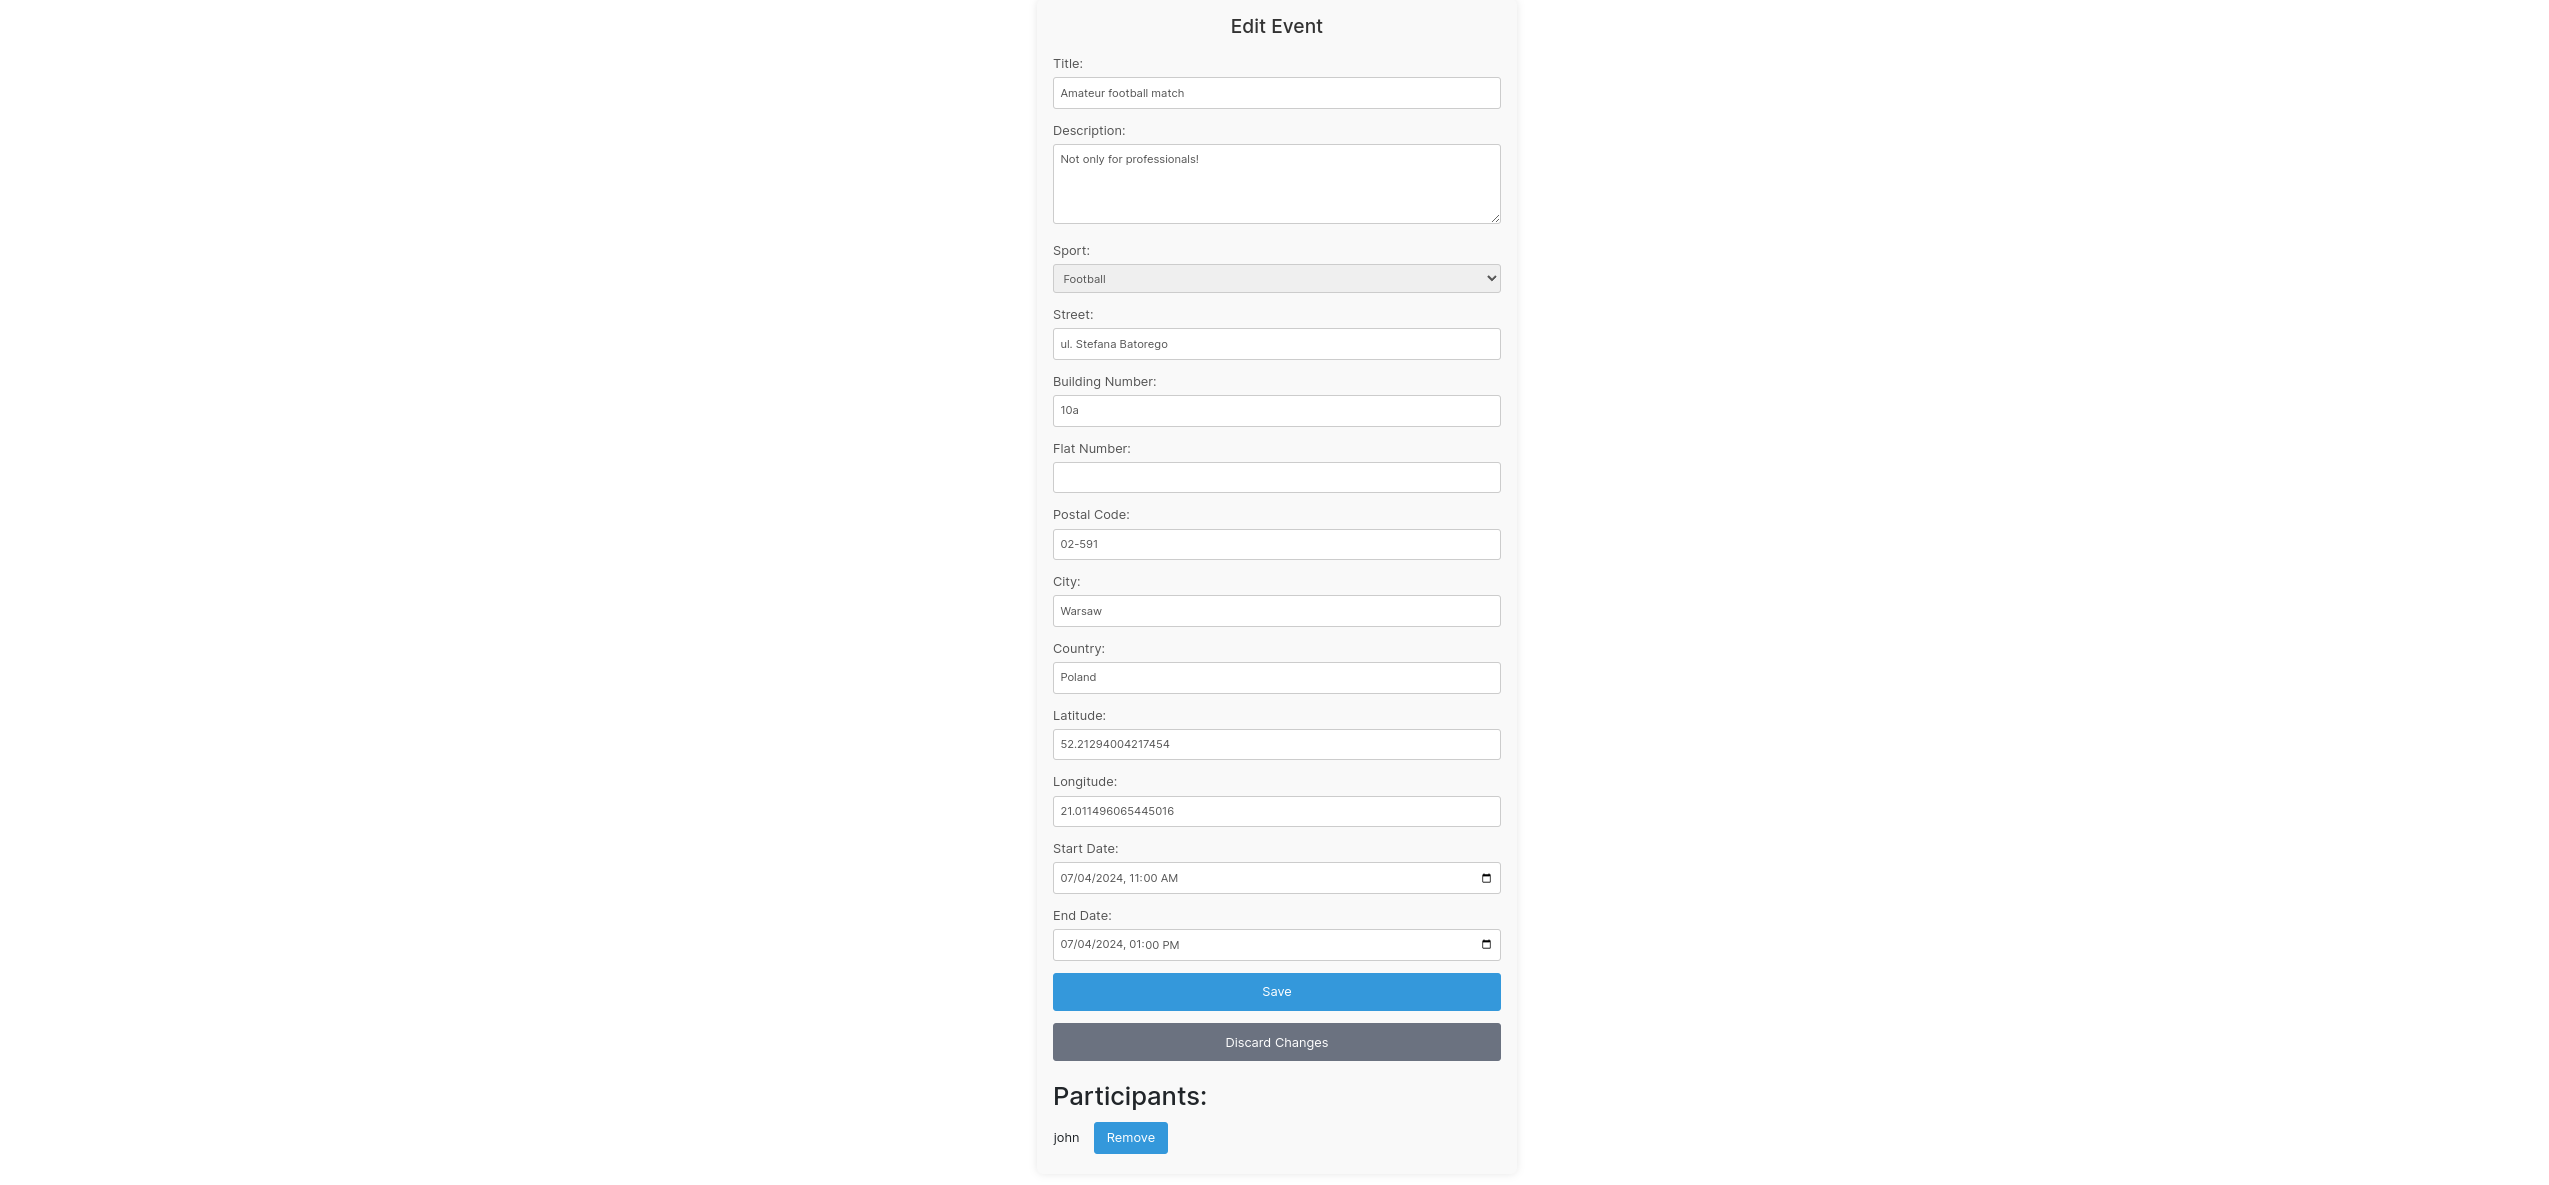
\includegraphics[width=1\linewidth]{pages/edit_event.png}
    \caption{Formularz edycji}
\end{figure}

\subsection{Usuwanie uczestników z utworzonego wydarzenia}

Aby usunąć zapisanego uczestnika z utworzonego wydarzenia, należy wejść do formularza edycji wydarzenia i kliknąć przycisk \textit{Remove} przy wybranym użytkowniku.

\begin{figure} [H]
    \centering
    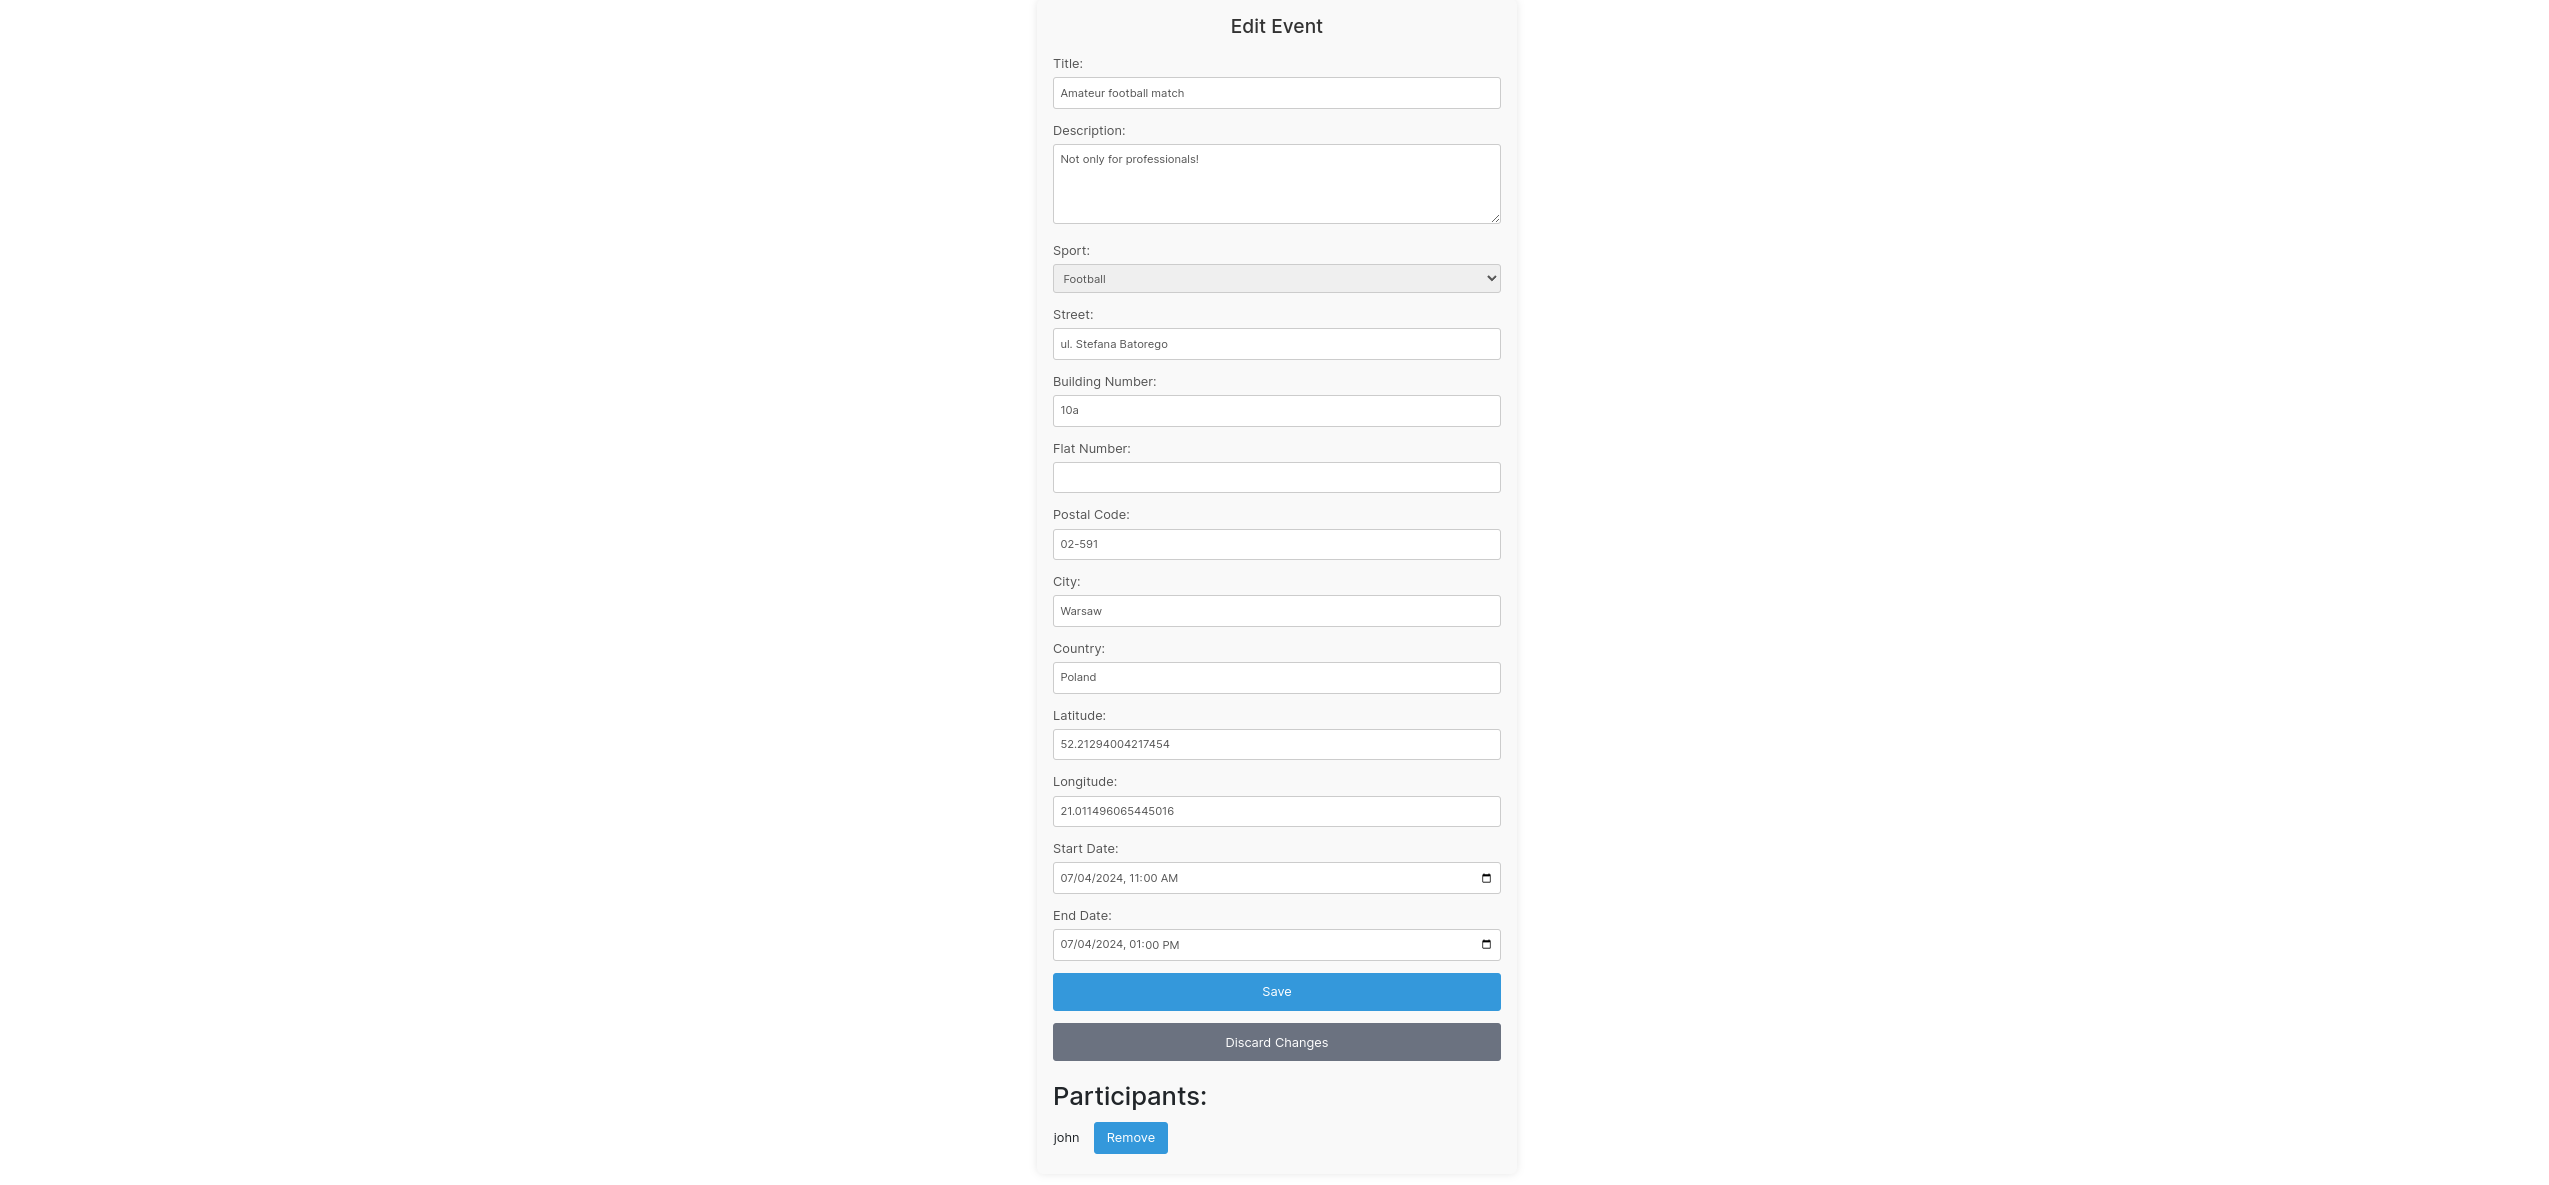
\includegraphics[width=1\linewidth]{pages/edit_event.png}
    \caption{Formularz edycji}
\end{figure}

\subsection{Usuwanie utworzonego wydarzenia}

Aby usunąć utworzone wydarzenie, należy wejść na jego stronę, a następnie kliknąć przycisk \textit{Delete Event}, po czym zostanie ukazany popup informujący o pomyślnym usunięciu wydarzenia, po czym użytkownik zostanie przeniesiony na stronę główną.

\begin{figure} [H]
    \centering
    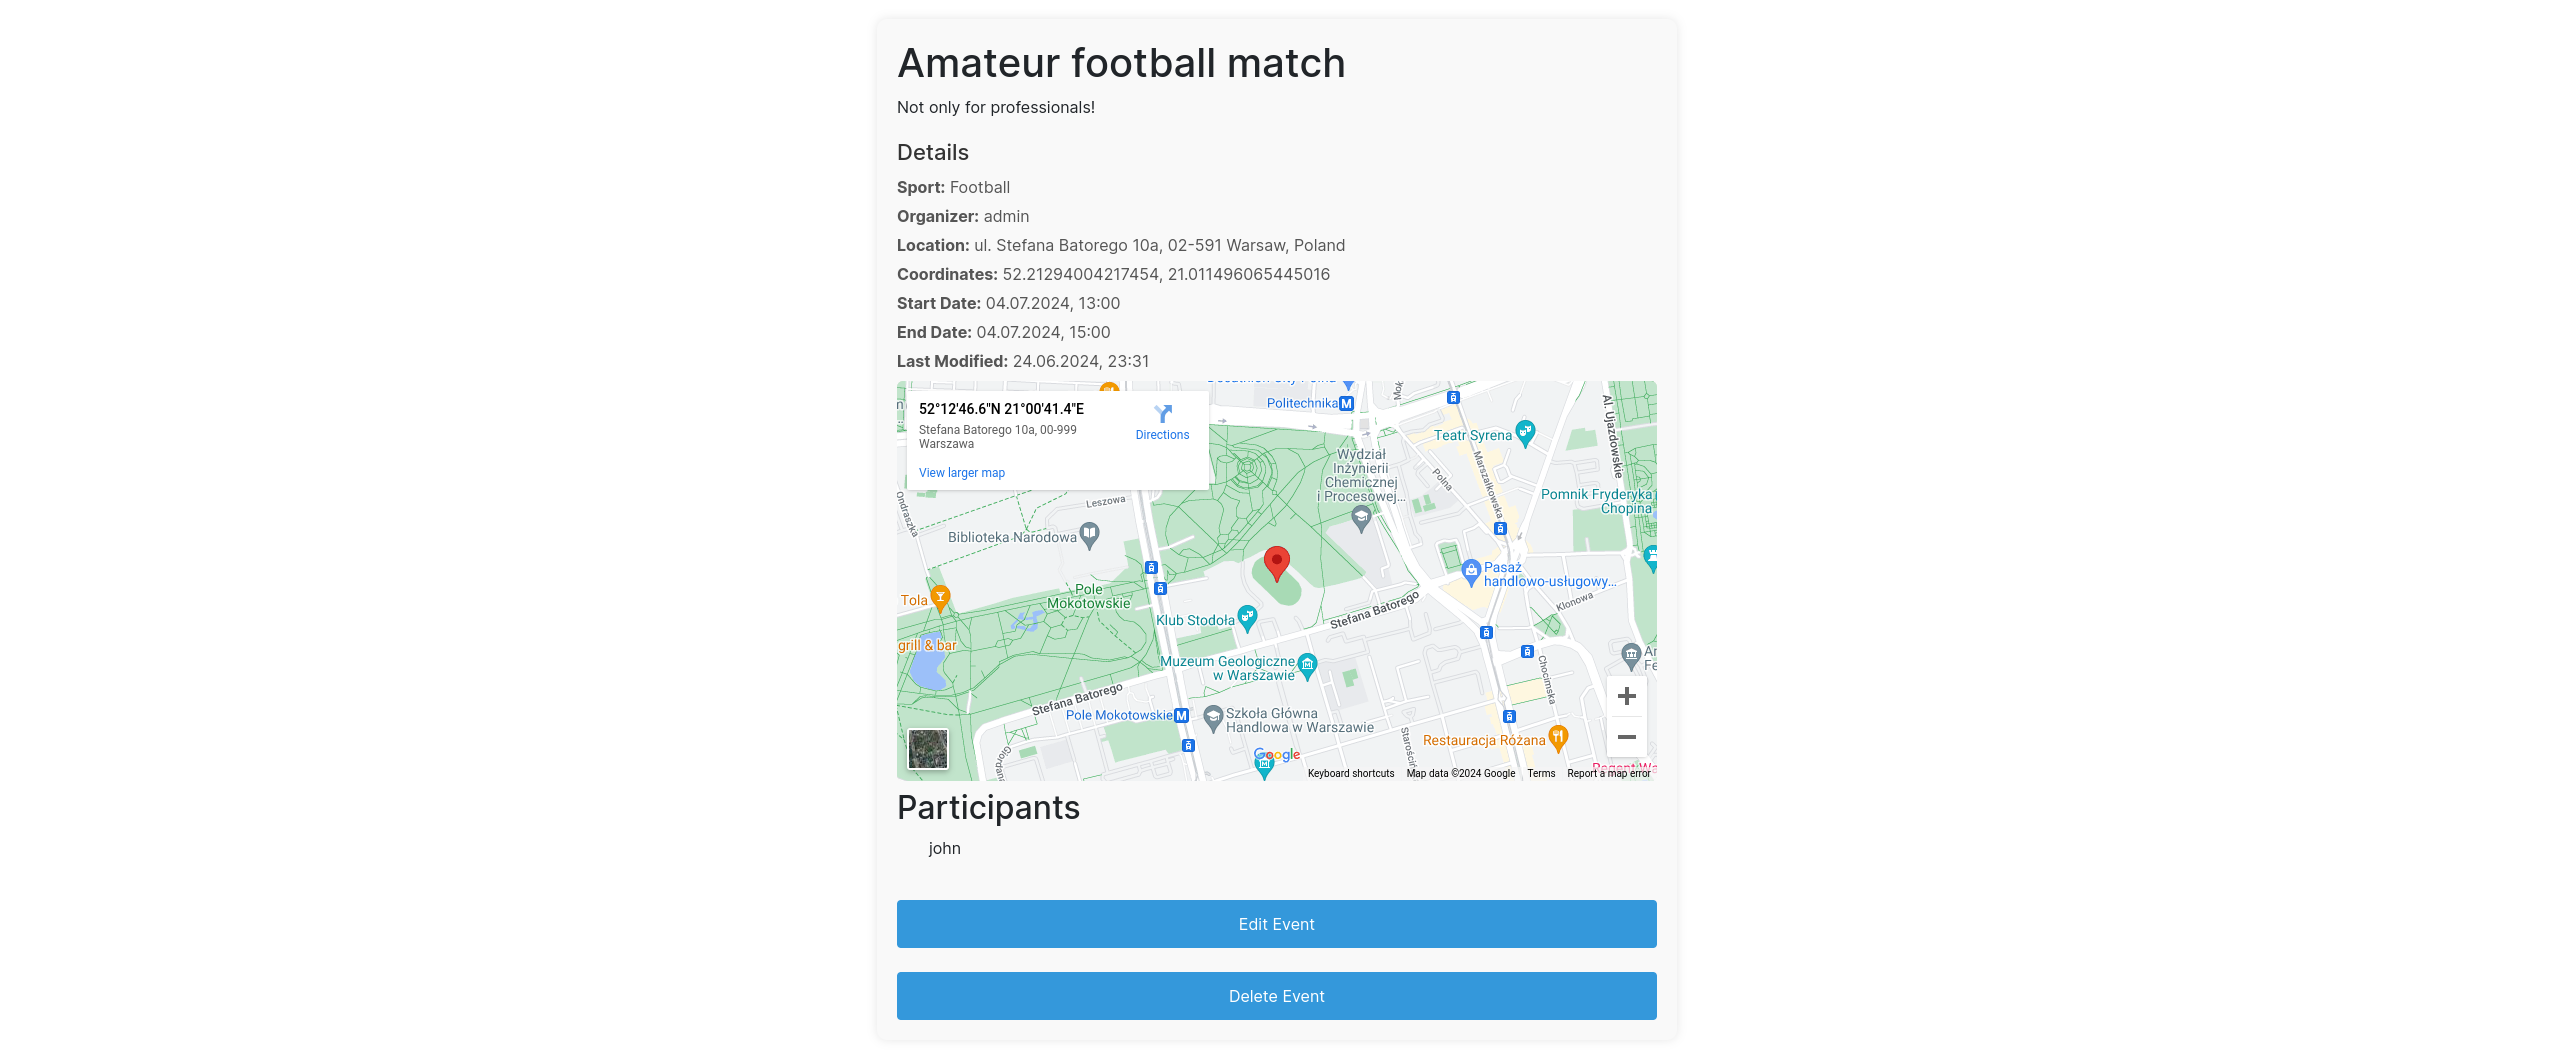
\includegraphics[width=1\linewidth]{pages/my_event.png}
    \caption{Strona utworzonego wydarzenia}
\end{figure}

\subsection{Wylogowanie się}

Aby się wylogować, należy kliknąć przycisk \textit{Sign out} na stronie głównej.

\end{document}
